%This file is just a wrapper. Please, edit the files for your chapter in chapters/chapter1/.
%Don't worry, we will put your chapter in the correct place when assemble the book.

\documentclass[krantz1,ChapterTOCs]{krantz}
\usepackage{fixltx2e,fix-cm}
\usepackage{amssymb}
\usepackage{amsmath}
\usepackage{graphicx}
\usepackage{subfigure}
\usepackage{makeidx}
\usepackage{multicol}

%\usepackage[dvips]{hyperref}

\frenchspacing
\tolerance=5000

\makeindex

\newtheorem{theorem}{Theorem}
\newtheorem{exercise}{Exercise}[chapter]
\newtheorem{example}{Example}
\newtheorem{definition}{Definition}
\newtheorem{proof}{Proof}
 %place custom commands and macros here

\begin{document}

\frontmatter

\title{Quantitative Approaches to Evaluating Climate Change Impacts... 
%in Socio-Environmental Systems, Public Health, and Insurance\\
%{\Large(Applied Environmental Statistics Series)}
}
\author{Yours Truly}

\maketitle

%\cleardoublepage
\thispagestyle{empty}
\vspace*{\stretch{1}}
\begin{center}
\Large\itshape
To my dog\\
and my cat.
\end{center}
\vspace{\stretch{2}}
%\cleardoublepage
\setcounter{page}{7} %previous pages will be reserved for frontmatter to be added in later.
\tableofcontents
%\chapter*{Foreword}
I am delighted to introduce the first book on Multimedia Data Mining.  When I came to know about this book project undertaken by two of the most active young researchers in the field, I was pleased that this book is coming in early stage of a field that will need it more than most fields do.  In most emerging research fields, a book can play a significant role in bringing some maturity to the field.  Research fields advance through research papers.  In research papers, however, only a limited perspective could be provided about the field, its application potential, and the techniques required and already developed in the field.  A book gives such a chance.  I liked the idea that there will be a book that will try to unify the field by bringing in disparate topics already available in several papers that are not easy to find and understand.  I was supportive of this book project even before I had seen any material on it.  The project was a brilliant and a bold idea by two active researchers.  Now that I have it on my screen, it appears to be even a better idea.  

Multimedia started gaining recognition in 1990s as a field.  Processing, storage, communication, and capture and display technologies had advanced enough that researchers and technologists started building approaches to combine information in multiple types of signals such as audio, images, video, and  text.  Multimedia computing and communication techniques recognize correlated information in multiple sources as well as insufficiency of information in any individual source.    By properly selecting sources to provide complementary information, such systems aspire, much like human perception system, to create a holistic picture of a situation using only partial information from separate sources.

Data mining is a direct outgrowth of progress in data storage and processing speeds.  When it became possible to store large volume of data and run different statistical computations to explore all possible and even unlikely correlations among data, the field of data mining was born.  Data mining allowed people to hypothesize relationships among data entities and explore support for those.  This field has been put to applications in many diverse domains and keeps getting more applications.  In fact many new fields are direct outgrowth of data mining and it is likely to become a powerful computational tool.\vadjust{\vfill\pagebreak}



%\chapter*{Preface}
Approximately 17 million people in the USA (6{\%} of the
population) and 140 million people worldwide (this number is
expected to rise to almost 300 million by the year 2025) suffer
from \textit{diabetes mellitus}. Currently, there a few dozens of
commercialised devices for detecting blood glucose levels [1].
However, most of them are invasive. The development of a
noninvasive method would considerably improve the quality of life
for diabetic patients, facilitate their compliance for glucose
monitoring, and reduce complications and mortality associated with
this disease. Noninvasive and continuous monitoring of glucose
concentration in blood and tissues is one of the most challenging
and exciting applications of optics in medicine. The major
difficulty in development and clinical application of optical
noninvasive blood glucose sensors is associated with very low
signal produced by glucose molecules. This results in low
sensitivity and specificity of glucose monitoring by optical
methods and needs a lot of efforts to overcome this difficulty.

A wide range of optical technologies have been designed in
attempts to develop robust noninvasive methods for glucose
sensing. The methods include infrared absorption, near-infrared
scattering, Raman, fluorescent, and thermal gradient
spectroscopies, as well as polarimetric, polarization
heterodyning, photonic crystal, optoacoustic, optothermal, and
optical coherence tomography (OCT) techniques [1-31].

For example, the polarimetric quantification of glucose is based
on the phenomenon of optical rotatory dispersion, whereby a chiral
molecule in an aqueous solution rotates the plane of linearly
polarized light passing through the solution. The angle of
rotation depends linearly on the concentration of the chiral
species, the pathlength through the sample, and the molecule
specific rotation. However, polarization sensitive optical
technique makes it difficult to measure \textit{in vivo} glucose
concentration in blood through the skin because of the strong
light scattering which causes light depolarization. For this
reason, the anterior chamber of the eye has been suggested as a
sight well suited for polarimetric measurements, since scattering
in the eye is generally very low compared to that in other
tissues, and a high correlation exists between the glucose in the
blood and in the aqueous humor. The high accuracy of anterior eye
chamber measurements is also due to the low concentration of
optically active aqueous proteins within the aqueous humor.

On the other hand, the concept of noninvasive blood glucose
sensing using the scattering properties of blood and tissues as an
alternative to spectral absorption and polarization methods for
monitoring of physiological glucose concentrations in diabetic
patients has been under intensive discussion for the last decade.
Many of the considered  effects, such as changing of the size,
refractive index, packing, and aggregation of RBC under glucose
variation, are important for glucose monitoring in diabetic
patients. Indeed, at physiological concentrations of glucose,
ranging from 40 to 400 mg/dl, the role of some of the effects may
be modified, and some other effects, such as glucose penetration
inside the RBC and the followed hemoglobin glycation, may be
important [30-32].

Noninvasive determination of glucose was attempted using light
scattering of skin tissue components measured by a
spatially-resolved diffuse reflectance or NIR fre\-quen\-cy-domain
reflectance techniques. Both approaches are based on change in
glucose concentration, which affects the refractive index mismatch
between the interstitial fluid and tissue fibers, and hence
reduces scattering coefficient. A glucose clamp experiment showed
that reduced scattering coefficient measured in the visible range
qualitatively tracked changes in blood glucose concentration for
the volunteer with diabetes studied.




\listoffigures
\listoftables
%%%\twocolumn
\chapter*{Contributors}

\begin{multicols}{2}
\contributor{Michael Aftosmis}{NASA Ames Research Center}{Moffett Field, California}

\contributor{Pratul K. Agarwal}{Oak Ridge National Laboratory}{Oak Ridge, Tennessee}

\contributor{Sadaf R. Alam}{Oak Ridge National Laboratory}{Oak Ridge, Tennessee}

\contributor{Gabrielle Allen}{Louisiana State University}{Baton Rouge, Louisiana}

\contributor{Martin Sandve Aln{\ae}s}{Simula Research Laboratory and University of Oslo, Norway}{Norway}

\contributor{Steven F. Ashby} {Lawrence Livermore National Laboratory}{Livermore, California}

\contributor{David A. Bader} {Georgia Institute of Technology}{Atlanta, Georgia}

\contributor{Benjamin Bergen} {Los Alamos National Laboratory}{Los Alamos, New Mexico}

\contributor{Jonathan W. Berry} {Sandia National Laboratories}{Albuquerque, New Mexico}

\contributor{Martin Berzins}{University of Utah}{Salt Lake City, Utah}

\contributor{Abhinav Bhatele}{University of Illinois}{Urbana-Champaign, Illinois}

\contributor{Christian Bischof} {RWTH Aachen University}{Germany}

\contributor{Rupak Biswas} {NASA Ames Research Center}{Moffett Field, California}\vspace*{5pt}

\contributor{Eric Bohm} {University of Illinois}{Urbana-Champaign, Illinois}\vspace*{5pt}

\contributor{James Bordner} {University of California, San Diego}{San Diego, California}\vspace*{5pt}

\contributor{George Bosilca} {University of Tennessee}{Knoxville, Tennessee}\vspace*{5pt}

\contributor{Greg L. Bryan} {Columbia University}{New York, New York}\vspace*{5pt}

\contributor{Marian Bubak} {AGH University of Science and Technology}{
Krak{\'o}w, Poland}\vspace*{5pt}

\contributor{Andrew Canning}{Lawrence Berkeley National
Laboratory}{Berkeley, California}

\contributor{Jonathan Carter} {Lawrence Berkeley National
Laboratory}{Berkeley, California}

\contributor{Zizhong Chen} {Jacksonville State University}{Jacksonville,
Alabama}

\contributor{Joseph R. Crobak} {Rutgers, The State University of New
Jersey}{Piscataway, New Jersey}

\contributor{Roxana E. Diaconescu} {Yahoo! Inc.}{Burbank, California}

\contributor{Peter Diener}
{Louisiana State University}{Baton Rouge, Louisiana}

\contributor{Jack J. Dongarra} {University of Tennessee, Knoxville, 
Oak Ridge National Laboratory, and}{University of Manchester}

\contributor{John B. Drake} {Oak Ridge National Laboratory}{Oak Ridge,
Tennessee}

\contributor{Kelvin K. Droegemeier} {University of Oklahoma}{Norman,
Oklahoma}

\contributor{St{\'e}phane Ethier} {Princeton University}{Princeton, New
Jersey}

\contributor{Christoph Freundl}
{Friedrich--Alexander--Universit{\"a}t}{Erlangen, Germany}

\contributor{Karl F{\"u}rlinger} {University of Tennessee}{Knoxville,
Tennessee}

\contributor{Al Geist} {Oak Ridge National Laboratory}{Oak Ridge,
Tennessee}

\contributor{Michael Gerndt} {Technische Universit{\"a}t
M{\"u}nchen}{Munich, Germany}

\contributor{Tom Goodale}
{Louisiana State University}{Baton Rouge, Louisiana}

\contributor{Tobias Gradl}
{Friedrich--Alexander--Universit{\"a}t}{Erlangen, Germany}

\contributor{William D. Gropp} {Argonne National Laboratory}{Argonne,
Illinois}

\contributor{Robert Harkness} {University of California, San
Diego}{San Diego, California}

\contributor{Albert Hartono} {Ohio State University}{Columbus, Ohio}

\contributor{Thomas C. Henderson} {University of Utah}{Salt Lake City,
Utah}

\contributor{Bruce A. Hendrickson} {Sandia National
Laboratories}{Albuquerque, New Mexico}

\contributor{Alfons G. Hoekstra} {University of Amsterdam}{Amsterdam,
The Netherlands}

\contributor{Philip W. Jones} {Los Alamos National Laboratory}{Los
Alamos, New Mexico}

\contributor{Laxmikant Kal{\'e}} {University of
Illinois}{Urbana-Champaign, Illinois}

\contributor{Shoaib Kamil} {Lawrence Berkeley National
Laboratory}{Berkeley, California}

\contributor{Cetin Kiris} {NASA Ames Research Center}{Moffett Field,
California}

\contributor{Uwe K{\"u}ster} {University of Stuttgart}{Stuttgart,
Germany}

\contributor{Julien Langou} {University of Colorado}{Denver, Colorado}

\contributor{Hans Petter Langtangen}
{Simula Research Laboratory and}{University of Oslo, Norway}

\contributor{Michael Lijewski} {Lawrence Berkeley National
Laboratory}{Berkeley, California}

\contributor{Anders Logg}
{Simula Research Laboratory and}{University of Oslo, Norway}

\contributor{Justin Luitjens} {University of Utah}{Salt Lake City, Utah}

\contributor{Kamesh Madduri} {Georgia Institute of Technology}{Atlanta,
Georgia}

\contributor{Kent-Andre Mardal}
{Simula Research Laboratory and}{University of Oslo, Norway}

\contributor{Satoshi Matsuoka} {Tokyo Institute of Technology}{Tokyo,
Japan}

\contributor{John M. May} {Lawrence Livermore National
Laboratory}{Livermore, California}

\contributor{Celso L. Mendes} {University of Illinois}{Urbana-Champaign,
Illinois}

\contributor{Dieter an Mey} {RWTH Aachen University}{Germany}

\contributor{Tetsu Narumi} {Keio University}{Japan}

\contributor{Michael L. Norman} {University of California, San
Diego}{San Diego, California}

\contributor{Boyana Norris} {Argonne National Laboratory}{Argonne,
Illinois}

\contributor{Yousuke Ohno} {Institute of Physical and Chemical Research
(RIKEN)}{Kanagawa, Japan}

\contributor{Leonid Oliker} {Lawrence Berkeley National
Laboratory}{Berkeley, California}

\contributor{Brian O'Shea} {Los Alamos National Laboratory}{Los Alamos,
New Mexico}

\contributor{Christian D. Ott}
{University of Arizona}{Tucson, Arizona}

\contributor{James C. Phillips} {University of
Illinois}{Urbana-Champaign, Illinois}

\contributor{Simon Portegies Zwart} {University of
Amsterdam,}{Amsterdam, The Netherlands}

\contributor{Thomas Radke}
{Albert-Einstein-Institut}{Golm, Germany}

\contributor{Michael Resch} {University of Stuttgart}{Stuttgart,
Germany}

\contributor{Daniel Reynolds} {University of California, San Diego}{San
Diego, California}

\contributor{Ulrich R{\"u}de}
{Friedrich--Alexander--Universit{\"a}t}{Erlangen, Germany}

\contributor{Samuel Sarholz}
{RWTH Aachen University}{Germany}

\contributor{Erik Schnetter}
{Louisiana State University}{Baton Rouge, Louisiana}

\contributor{Klaus Schulten} {University of Illinois}{Urbana-Champaign,
Illinois}

\contributor{Edward Seidel}
{Louisiana State University}{Baton Rouge, Louisiana}

\contributor{John Shalf} {Lawrence Berkeley National
Laboratory}{Berkeley, California}

\contributor{Bo-Wen Shen} {NASA Goddard Space Flight Center}{Greenbelt,
Maryland}

\contributor{Ola Skavhaug}
{Simula Research Laboratory and}{University of Oslo, Norway}

\contributor{Peter M.A. Sloot} {University of Amsterdam}{Amsterdam, The
Netherlands}

\contributor{Erich Strohmaier} {Lawrence Berkeley National
Laboratory}{Berkeley, California}

\contributor{Makoto Taiji} {Institute of Physical and Chemical Research
(RIKEN)}{Kanagawa, Japan}

\contributor{Christian Terboven}
{RWTH Aachen University,}{Germany}

\contributor{Mariana Vertenstein} {National Center for Atmospheric
Research}{Boulder, Colorado}

\contributor{Rick Wagner} {University of California, San Diego}{San
Diego, California}

\contributor{Daniel Weber} {University of Oklahoma}{Norman, Oklahoma}

\contributor{James B. White, III} {Oak Ridge National Laboratory}{Oak
Ridge, Tennessee}

\contributor{Terry Wilmarth} {University of Illinois}{Urbana-Champaign,
Illinois}

\end{multicols}
%\chapter*{Symbols}
\begin{symbollist}{000000}
\symbolentry{$\alpha$}{To solve the generator maintenance scheduling, in the  past, several mathematical techniques have  been applied.}
\symbolentry{$\sigma^2$}{These include integer programming, integer linear programming, dynamic programming, branch and bound etc.}
\symbolentry{$\sum$}{Several heuristic search algorithms have also been developed. In recent years expert systems,}
\symbolentry{$abc$}{fuzzy approaches, simulated annealing and genetic algorithms have also been tested.}
\symbolentry{$\theta\sqrt{abc}$}{This paper presents a survey of the literature}
\symbolentry{$\zeta$}{ over the past fifteen years in the generator}
\symbolentry{$\partial$}{maintenance scheduling. The objective is to}
\symbolentry{sdf}{present a clear picture of the available recent literature}
\symbolentry{ewq}{of the problem, the constraints and the other aspects of}
\symbolentry{bvcn}{the generator maintenance schedule.}
\end{symbollist}

\mainmatter

\part{Ecosystem-base Impacts of Climate Change}
\chapterauthor{Author Name}{Author Affiliation}
\chapterauthor{Second Author}{Second Author Affiliation}
\chapter{Basic Concepts}

A component part for an electronic item is
manufactured at one of three different factories, and then delivered to
the main assembly line.Of the total number supplied, factory A supplies
50\%, factory B 30\%, and factory C 20\%. Of the components
manufactured at factory A, 1\% are faulty and the corresponding
proportions for factories B and C are 4\% and 2\% respectively. A
component is picked at random from the assembly line. What is the
probability that it is faulty?

\section{Introduction}\label{intro}
The term reliability usually refers to the probability that a
component or system will operate satisfactorily either at any particular
instant at which it is required or for a certain length of
time. Fundamental to quantifying reliability s a knowledge of how to
define, assess and combine probabilities \cite{Bontempi2005Adaptive}. This may hinge on identifying the
form of the variability which is nherent n most processes. If all
components had a fixed known lifetime there would be no need to model
reliability.

\begin{enumerate}[1.]
\item A component part for an electronic item is
manufactured at one of three different factories.

\item A component part $x$ for an electronic item is
manufactured at one of three different factories.
\begin{enumerate}
\item A component part for an electronic item is
manufactured at one of three different factories.

\item A component part $x$ for an electronic item is
manufactured at one of three different factories.
\begin{enumerate}[iv.]
\item A component part for an electronic item is
manufactured at one of three different factories.

\item A component part $x$ for an electronic item is
manufactured at one of three different factories.

\item A component part for an electronic item is
manufactured at one of three different factories.

\item A component part 1, 2, 3, 4 for an electronic item is
manufactured at one of three different factories.

\item A component part for enumerate list of an electronic item is
manufactured at one of three different factories.

\end{enumerate}

\item A component part for an electronic item is
manufactured at one of three different factories.

\item A component part 1, 2, 3, 4 for an electronic item is
manufactured at one of three different factories.

\item A component part for enumerate list of an electronic item is
manufactured at one of three different factories.

\end{enumerate}

\item A component part for an electronic item is
manufactured at one of three different factories.

\item A component part 1, 2, 3, 4 for an electronic item is
manufactured at one of three different factories.

\item A component part for enumerate list of an electronic item is
manufactured at one of three different factories.

\end{enumerate}

\subsection{A component part}
A component part for an electronic item is
manufactured at one of three different factories, and then delivered to
the main assembly line.Of the total number supplied, factory A supplies
50\%, factory B 30\%, and factory C 20\%. Of the components
manufactured at factory A, 1\% are faulty and the corresponding
proportions for factories B and C are 4\% and 2\% respectively. A
component is picked at random from the assembly line. What is the
probability that it is faulty \cite{ilyas2004hsn}?
A component part for an electronic item is
manufactured at one of three different factories, and then delivered to
the main assembly line. Of the total number supplied, factory A supplies
50\%, factory B 30\%, and factory C 20\%. Of the components
manufactured at factory A, 1\% are faulty and the corresponding
proportions for factories B and C are 4\% and 2\% respectively. A
component is picked at random from the assembly line. What is the
probability that it is faulty?
A component part for an electronic item is
manufactured at one of three different factories, and then delivered to
the main assembly line.Of the total number supplied, factory A supplies
50\%, factory B 30\%, and factory C 20\%. Of the components
manufactured at factory A, 1\% are faulty and the corresponding
proportions for factories B and C are 4\% and 2\% respectively. A
component is picked at random from the assembly line. What is the
probability that it is faulty?

\begin{VF}
``A Process is a structured, measured set of activities designed to produce a specific output for a particular customer
or market---A process is thus a specific ordering of work activities across time and space, with a beginning, an end.
and clearly defined inputs and outputs: a structure for action.''

\VA{Thomas Davenport}{Senior Adjutant to the Junior Marketing VP}
\end{VF}


\begin{table}%1
%\noautomaticrules
\tabletitle{Now we are engaged $(a_g^a)$ $\big(a_g^a\big)$ in a great civil war, testing whether that
nation, or any nation so conceived.}%
\begin{tabular}{lccc}
\tch{Scene}    &\tch{Reg. fts.} &\tch{Hor. fts.} &\tch{Ver. fts.}\\
Ball &19, 221 &4, 598   &3, 200\\
Pepsi$^a$&46, 281 &6, 898 &5, 400\\
Keybrd$^b$   &27, 290 &2, 968 &3, 405\\
Pepsi    &14, 796 &9, 188 &3, 209\\
\end{tabular}
\end{table}

\textbf{MultiRelational $k$-Anonymity.} Most works on $k$-anonymity focus on anonymizing a single data table; however, a real-life \cite{diamantaras1996pcn} database usually contains multiple relational tables. This has proposed a privacy model called \emph{MultiR $k$-anonymity} to ensure $k$-anonymity on multiple relational tables. Their model assumes that a relational database contains a person-specific table $PT$ and a set of tables $T_1,\cdots,T_n$, where $PT$ contains a person identifier $Pid$ and some sensitive attributes, and $T_i$, for $1 \leq i \leq n$, contains some foreign keys, some attributes in $QID$, and sensitive attributes. The general privacy notion is to ensure that for each record owner $o$ contained in the join of all tables $PT \Join T_1 \Join \cdots \Join T_n$, there exists at least $k-1$ other record owners share the same $QID$ with $o$. It is important to emphasize that the $k$-anonymization is applied at the \emph{record owner} level, not at the \emph{record} level in traditional $k$-anonymity. This idea is similar to $(X,Y)$-anonymity, where $X=QID$ and $Y=\{Pid\}$.

Most works on $k$-anonymity focus on anonymizing a single data table; however, a real-life \cite{diamantaras1996pcn} database usually contains multiple relational tables. This has proposed a privacy model called \emph{MultiR $k$-anonymity} to ensure $k$-anonymity on multiple relational tables. Their model assumes that a relational database contains a person-specific table $PT$ and a set of tables $T_1,\cdots,T_n$, where $PT$ contains a person identifier $Pid$ and some sensitive attributes, and $T_i$, for $1 \leq i \leq n$, contains some foreign keys, some attributes in $QID$, and sensitive attributes. The general privacy notion is to ensure that for each record owner $o$ contained in the join of all tables $PT \Join T_1 \Join \cdots \Join T_n$, there exists at least $k-1$ other record owners share the same $QID$ with $o$. It is important to emphasize that the $k$-anonymization is applied at the \emph{record owner} level, not at the \emph{record} level in traditional $k$-anonymity. This idea is similar to $(X,Y)$-anonymity, where $X=QID$ and $Y=\{Pid\}$.

\begin{table}[b!]%2
\tabletitle[Short Table Caption]{Now we are engaged $(a_g^a)$ $\big(a_g^a\big)$ in a great civil war, testing whether that
nation, or any nation so conceived.}%}{%
\begin{tabular}{lccc}
\tch{Scene}    &\tch{Reg. fts.} &\tch{Hor. fts.} &\tch{Ver. fts.}\\
\multicolumn{4}{@{}l@{}}{\tsh{Table Head}}\\[3pt]\hline\\[-6pt]
Ball &19, 221 &4, 598   &3, 200\\
Pepsi &46, 281 &6, 898 &5, 400\\
Keybrd   &27, 290 &2, 968 &3, 405\\
Pepsi    &14, 796 &9, 188 &3, 209\\
\end{tabular}
\end{table}

% \begin{shadebox} %This doesn’t work with the pdftex engine -- see the manual.
% A component part for an electronic item is
% manufactured at one of three different factories, and then delivered to
% the main assembly line.Of the total number supplied, factory A supplies
% 50\%, factory B 30\%, and factory C 20\%. Of the components
% manufactured at factory A, 1\% are faulty and the corresponding
% proportions for factories B and C are 4\% and 2\% respectively. A
% component is picked at random from the assembly line. What is the
% probability that it is faulty?
% \end{shadebox}

In most literature on PPDP, they \cite{jolliffe2002pca} consider a more relaxed, yet more practical, notion of privacy protection by assuming limited attacker's background knowledge. Below, the term ``victim" refers to the record owner being linked. We can broadly classify linking models to two families.

\begin{extract}
A component part for an electronic item is \cite{hyvarinen2001ica}
manufactured at one of three different factories, and then delivered to
the main assembly line.Of the total number supplied, factory A supplies
50\%, factory B 30\%, and factory C 20\%. Of the components
manufactured at factory A, 1\% are faulty and the corresponding
proportions for factories B and C are 4\% and 2\% respectively.
\end{extract}


One family considers a privacy threat occurs when an attacker is able to link a record owner to a record in a published data table, to a sensitive attribute in a published data table, or to the published data table itself. We call them \emph{record linkage}, \emph{attribute linkage}, and \emph{table linkage}, respectively. In all types of linkages, we assume that the attacker knows the $QID$ of the victim. In record and attribute linkages, we further assume that the attacker knows the presence of the victim's record in the released table, and seeks to identify the victim's record and/or sensitive information from the table \cite{yao2002can}. In table linkage, the attack seeks to determine the present or absent of the victim's record in the released table. A data table is considered to privacy preserved if the table can effectively prevent the attacker from successfully performing these types of linkages on the table \cite{madden2002tta}. Sections~\ref{intro}-\ref{sec:reclinkage} study this family of privacy models.
\begin{equation}
\mbox{var}\widehat{\Delta} = \sum_{j = 1}^t \sum_{k = j+1}^t
\mbox{var}\,(\hat{\alpha}_j - \hat{\alpha}_k)  = \sum_{j = 1}^t
\sum_{k = j+1}^t \sigma^2(1/n_j + 1/n_k). \label{2delvart2}
\end{equation}


An obvious measure of imbalance is just the difference in the
number of times the two treatments are allocated
\begin{equation}
D_n = \mathcal{M}|n_A - n_B|. \label{2deffD}
\end{equation}
For rules such as deterministic allocation, for which the expected
value of this difference can be calculated, we obtain the population
value ${\cal D}_n$.

\begin{shortbox}
\Boxhead{Box Title Here}
Another family aims at achieving the \emph{uninformative principle}: The published table should provide the attacker with little additional information beyond the background knowledge. There should not be a large difference between the prior and posterior beliefs; otherwise, there is a privacy threat~\cite{jain2004ass, jolliffe2002pca}. Many privacy models in this family are designed for statistical database and do not distinguish attributes in $T$ into $QID$, but some of them could also thwart record, attribute, and table linkages. Section~\ref{intro} studies this family of privacy models.

Let $m$ be a prime number. With the addition and multiplication as
defined above, $Z_m$ is a field.
\end{shortbox}

\begin{theorem}\label{1th:Z_m}
Let $m$ be a prime number. With the addition and multiplication as
defined above, $Z_m$ is a field.
\end{theorem}

\begin{proof}
Most of the proof of this theorem is routine.  It is clear that $0\in Z_m$
and $1\in Z_m$ are the
zero element and identity element. If $a\in Z_m$ and $a\ne 0$, then $m-a$
is the additive inverse of $a$. If $a\in Z_m$ and $a\ne 0$, then the
greatest common divisor of $a$ and $m$ is 1, and hence
there exist integers $s$ and $t$ such that $sa+tm=1$. Thus $sa=1 -tm$ is
congruent to 1 modulo $m$. Let $s^*$ be the integer in $Z_m$
congruent to $s$
modulo $m$. Then we also have $s^*a\equiv 1\  \mbox{mod}\ m$. Hence $s^*$
is
the multiplicative inverse of $a$ modulo $m$. Verification of the rest of
the field properties is now routine.\end{proof}



\section{Record Linkage Model}\label{sec:reclinkage}

In the privacy attack of \emph{record linkage}, some value $qid$ on $QID$ identifies a small number of records in the released table $T$,
called a \emph{group}. If the victim's $QID$ matches the value
$qid$, the victim is vulnerable to being linked to the small
number of records in the group \cite{madden2005taq}. In this case, the attacker faces
only a small number of possibilities for the victim's record, and
with the help of additional knowledge, there is a chance that the
attacker could uniquely identify the victim's record from the
group.


%%%\begin{table}
%%%    \tabletitle{Examples for illustrating attacks}
%%%    \begin{tabular}{|c|c|c|c|}
%%%        \hline
%%%        \textbf{Job} & \textbf{Sex} & \textbf{Age} & \textbf{Disease} \\
%%%        \hline
%%%        Engineer & Male & 35 & Hepatitis \\
%%%        Engineer & Male & 38 & Hepatitis \\
%%%        Lawyer & Male & 38 & HIV \\
%%%        Writer & Female & 30 & Flu \\
%%%        Writer & Female & 30 & HIV \\
%%%        Dancer & Female & 30 & HIV \\
%%%        Dancer & Female & 30 & HIV \\
%%%        \hline
%%%    \end{tabular}
%%%    \label{table:rawpatient}
%%%\end{table}



\subsection{A component part}
A component part for an electronic item is
manufactured at one of three different factories, and then delivered to
the main assembly line.Of the total number supplied, factory A supplies
50\%, factory B 30\%, and factory C 20\%. Of the components
manufactured at factory A, 1\% are faulty and the corresponding
proportions for factories B and C are 4\% and 2\% respectively. A
component is picked at random from the assembly line. What is the
probability that it is faulty?



\begin{figure}

\includegraphics[width=350pt, height=200pt]{chapters/chapter1/figures/cat.eps}
%%\centerline{\epsfig{/Chapters/chapter1/figures/cat.eps,width=.8\textheight,height=.4\textwidth}}
\caption[List of figure caption goes here]{Figure caption goes here.}
\end{figure}



\begin{figure}[htb]

\includegraphics[width=200pt, height=200pt]{chapters/chapter1/figures/cat}
%%\centerline{\epsfig{figure=cat.eps,width=.5\textheight,height=.4\textwidth}}
\caption[Short figure caption]{Figure caption goes here. Figure caption goes here.
Figure caption goes here. Figure caption goes here. Figure caption goes here.
Figure caption goes here.}
\end{figure}





\begin{figure}
\begin{center}
\subfigure[\label{f8a}]{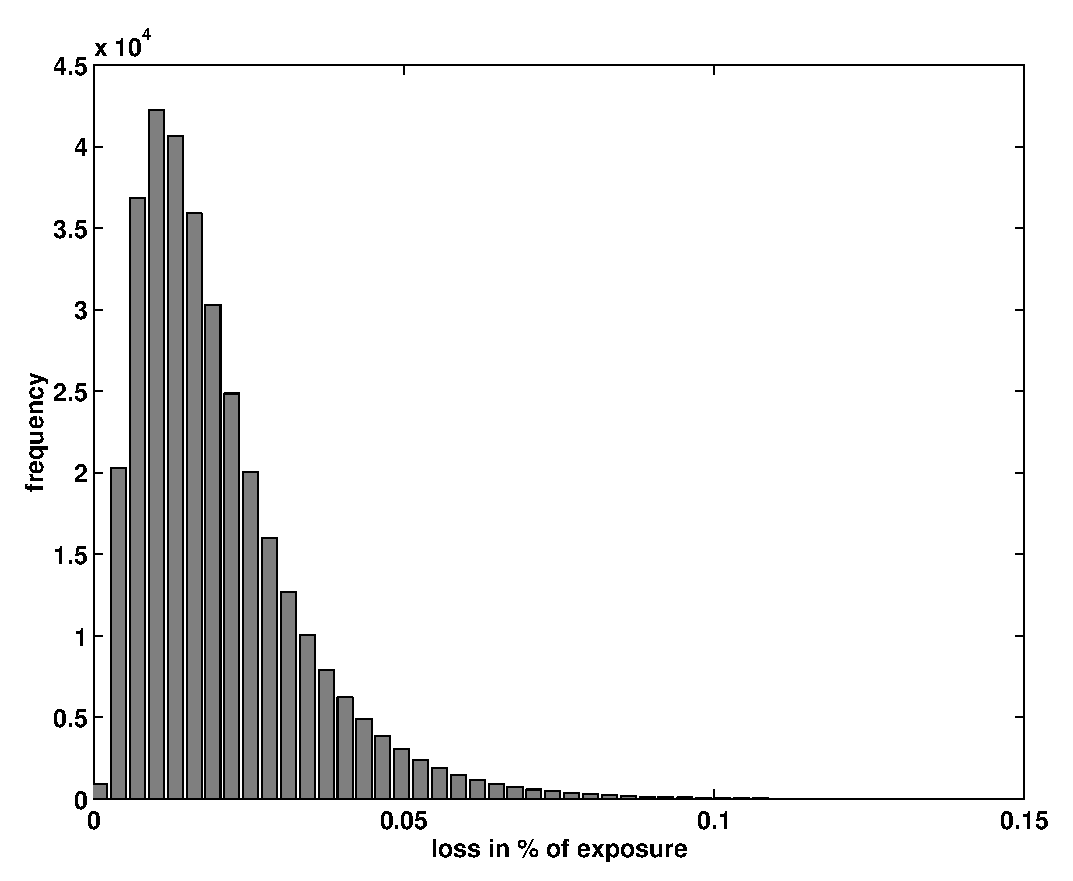
\includegraphics[angle=90,width=7cm,height=7cm,angle=-90]{chapters/chapter1/figures/Histogram.eps}}
\subfigure[\label{f8b}]{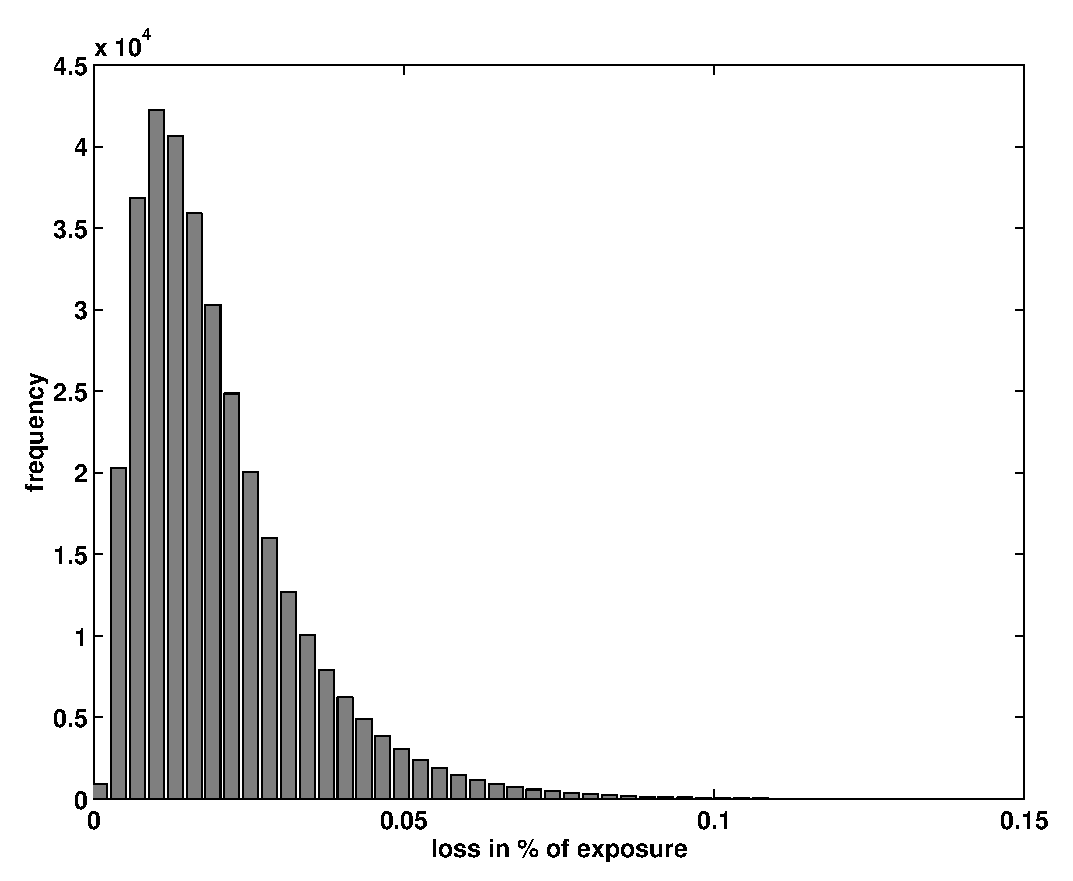
\includegraphics[angle=90,width=7cm,height=7cm,angle=-90]{chapters/chapter1/figures/Histogram.eps}}
\end{center}
\caption[The bar charts depict the different risk contributions]{The bar charts depict the different risk contributions (top: 99\% quantile, bottom: 99.9\% quantile) of the business areas of a bank. The black bars
are based on a Var/Covar approach, the white ones correspond to shortfall risk.}
\end{figure}

\subsubsection{H3 A component part }
A component part for an electronic item is
manufactured at one of three \cite{mardia1979ma} different factories, and then delivered to
the main assembly line.Of the total number supplied, factory A supplies
50\%, factory B 30\%, and factory C 20\%. Of the components
manufactured at factory A, 1\% are faulty and the corresponding
proportions for factories B and C are 4\% and 2\% respectively. A
component is picked at random from the assembly line. What is the
probability that it is faulty?


A fundamental notion \cite{yao2002can} is that of a\index{subspace}\index{vector
space!subspace of} subspace of $F^n$. Let $V$ be a nonempty subset of
$F^n$. Then $V$ is a {\it subspace} of $F^n$ provided $V$ is closed
under vector addition and scalar multiplication, that is,
\begin{enumerate}
\item[\rm (a)] For all $u$ and $v$ in $V$, $u+v$ is
also in $V$.
\item[\rm (b)] For all $u$ in $V$ and $c$ in $F$, $cu$ is
in $V$.
\end{enumerate}
Let $u$ be in the subspace $V$. Because $0u=0$,
it follows that the zero vector is in $V$. Similarly, $-u$ is in $V$
for all $u$ in $V$. A simple example of a subspace of $F^n$ is the set
of all vectors $(0,a_2,\ldots,a_n)$ with first coordinate equal to 0.
The zero vector itself is a subspace.

\begin{definition}\label{1def:linearcomb}{\rm
Let $u^{(1)},u^{(2)},\ldots,u^{(m)}$ be vectors in $F^n$, and let
$c_1,c_2,\ldots,c_m$ be scalars. Then the vector
\[c_1u^{(1)}+c_2u^{(2)}+\cdots+c_mu^{(m)}\]
is called a {\it linear combination} \index{linear combination} of $u^{(1)},u^{(2)},\ldots,u^{(m)}$.
If $V$ is a subspace of $F^n$, then $V$ is closed under vector addition and
scalar multiplication, and it follows easily by induction that a
linear combination of vectors in $V$ is also a vector in $V$. Thus
{\it subspaces
are closed under linear combinations}; in fact, this can be taken as the
defining property of subspaces.
The vectors $u^{(1)},u^{(2)},\ldots,u^{(m)}$ {\it span} $V$ \index{spanning set}
(equivalently, form a {\it spanning set} of $V$) provided every vector in
$V$
is a linear combination of $u^{(1)},u^{(2)},\ldots,u^{(m)}$. The zero
vector can be written as a linear combination of
$u^{(1)},u^{(2)},\ldots,u^{(m)}$ with all scalars equal to 0; this is a
{\it trivial linear combination}.\index{linear combination!trivial} The vectors
$u^{(1)},u^{(2)},\ldots,u^{(m)}$ are {\it linearly dependent} provided
there are scalars $c_1,c_2,\ldots,c_m$, not all of which are zero, such
that
\[c_1u^{(1)}+c_2u^{(2)}+\cdots+c_mu^{(m)}=0,\]
that is, the zero vector can be written as a {\it nontrivial linear \index{linear combination!nontrivial}
combination} of $u^{(1)},u^{(2)},\ldots,u^{(m)}$.
For example, the vectors $(1,4), (3,-1)$, and $(3,5)$ in $\Re^2$ are
linearly
dependent since
\[3(1,4)+1(3,-2)-2(3,5)=(0,0).\] Vectors are {\it linearly independent} provided  they are not linearly dependent.\index{linearly independent}
The vectors
$u^{(1)},u^{(2)},\ldots,u^{(m)}$ are a {\it basis} \index{basis} of $V$ provided they are
linearly independent and span $V$.
By an {\it ordered basis} \index{basis!ordered} we mean a basis in which the vectors of the basis are listed
in a specified order; to indicate that we have an ordered basis we write
$(u^{(1)},u^{(2)},\ldots,u^{(m)})$.
A spanning set $S$ of $V$ is a \index{spanning set!minimal} {\it minimal spanning set of $V$} provided that
each set
of vectors obtained from $S$ by removing a vector is not a spanning set
for $V$.
A linearly independent set $S$ of vectors of $V$ is a {\it maximal linearly \index{linearly independent!maximal}
independent set of vectors of $V$} provided that for each vector $w$ of
$V$ that
is not in $S$, $S\cup\{w\}$ is  linearly dependent (when this happens,
$w$ must be  a linear combination of the vectors in
$S$).\hfill{$\Box$}
}\end{definition}

In addition to matrix addition, subtraction, and multiplication, there is
one additional operation that we define now. It's perhaps the simplest of
them all. Let $A=[a_{ij}]$ be an $m$ by $n$ matrix and let $c$ be a
number \cite{hyvarinen2001ica}. Then the matrix $c\cdot A$, or simply $cA$, is the $m$ by $n$
matrix obtained by multiplying each entry of $A$ by $c$:
\[c A=[ca_{ij}].\]\index{matrix!scalar multiplication} \index{matrix!scalar multiple of}
The matrix $c A$ is called a {\it scalar multiple} of $A$.

\begin{VT1}

\VH{Think About It...}

Commonly thought of as the first modern computer, ENTAC was built in 1944. It took up more space than an 18-wheeler's
tractor trailer and weighed more than 17 Chevrolet Camaros. It consumed 140,000 watts of electricity while executing
up to 5,000 basic arithmetic operations per second. One of today's popular microprocessors, the 486, is built on a
tiny piece of silicon about the size of a dime.

\VT
With the continual expansion of capabilities, computing power will eventually exceed the capacity for human
comprehension or human control.

\VTA{The Information Revolution}{Business Week}
\end{VT1}


\section{Glossary}
\begin{Glossary}
\item[360 Degree Review] Performance review that includes feedback from superiors, peers, subordinates, and clients.
\item[Abnormal Variation] Changes in process performance that cannot be accounted for by typical day-to-day variation. Also referred to as
non-random variation.
\item[Acceptable Quality Level (AQL)] The minimum number of parts that must comply with quality standards, usually stated as a percentage.
\item[Activity] The tasks performed to change inputs into outputs.
\item[Adaptable] An adaptable process is designed to maintain effectiveness and efficiency as requirements change. The process is
deemed adaptable when there is agreement among suppliers, owners, and customers that the process will meet
requirements throughout the strategic period.
\end{Glossary}




%%This chapter was modified on 4/2/97.
%\setcounter{chapter}{1}
\chapter{Continuous Probability Densities}\label{chp 2}

\section{Simulation of Continuous Probabilities}\label{sec 2.1}

In this section we shall show how we can use computer simulations for
experiments that have a whole continuum\index{continuum} of possible outcomes.

\subsection*{Probabilities}

\begin{example}\label{exam 2.1.1}
We begin by constructing a spinner\index{spinner}, which consists of a circle of \emx {unit 
circumference} and a pointer as shown in Figure~\ref{fig 2.05}.  We pick a point on
the circle and label it 0, and then label every other point on the circle with the
distance, say $x$, from 0 to that point, measured counterclockwise.  The experiment consists of
spinning the pointer and recording the label of the point at the tip of the
pointer.  We let the random variable $X$ denote the value of this outcome.   The sample space
is clearly the interval $[0, 1)$.  We would like to construct a probability model in which
each outcome is equally likely to occur.
\par
If we proceed as we did in Chapter~\ref{chp 1} for experiments with a finite number of
possible outcomes, then we must assign the probability 0 to each outcome, since otherwise,
the sum of the probabilities, over all of the possible outcomes, would not equal 1.  (In
fact, summing an uncountable number of real numbers is a tricky business; in particular, 
in order for such a sum to have any meaning, at most countably many of the summands can be
different than 0.)  However, if all of the assigned probabilities are 0, then the sum is 0,
not 1, as it should be.
\putfig{2truein}{PSfig2-12arc}{A spinner.}{fig 2.05}
\par
In the next section, we will show how to construct a probability model in this situation. 
At present, we will assume that such a model can be constructed.  We will also assume that
in this model, if $E$ is an arc of the circle, and $E$ is of length $p$, then the model 
will assign the probability $p$ to $E$.  This means that if the pointer is spun, the
probability that it ends up pointing to a point in $E$ equals $p$, which is certainly a
reasonable thing to expect.
\par
To simulate this experiment on a computer is an easy matter.  Many computer software
packages have a function which returns a random real number in the interval $[0, 1]$. 
Actually, the returned value is always a rational number, and the values are determined by
an algorithm, so a sequence of such values is not truly random.  Nevertheless,
the sequences produced by such algorithms behave much like theoretically random sequences,
so we can use such sequences in the simulation of experiments.  On occasion, we will need
to refer to such a function.  We will call this function $rnd$\index{rnd}.
\end{example}

\subsection*{Monte Carlo Procedure and Areas}

It is sometimes desirable to estimate quantities whose exact values are difficult or 
impossible to calculate exactly.  In some of these cases, a procedure involving chance, called 
a \emx {Monte Carlo procedure}, can be used to provide such an estimate.

\begin{example}\label{exam 2.1.2}
In this example we show how simulation can be used to estimate areas
\index{area, estimation of} of
plane figures.  Suppose that we program our computer to provide a pair $(x,y)$ or
numbers, each chosen independently at random from the interval $[0,1]$.  Then
we can interpret this pair $(x,y)$ as the coordinates of a point chosen \emx {at
random} from the unit square.  Events are subsets of the unit square. 
Our experience with Example~\ref{exam 2.1.1} suggests that the point is
equally likely to fall in subsets of equal area.  Since the total area of the
square is 1, the probability of the point falling in a specific subset $E$ of
the unit square should be equal to its area.  Thus, we can estimate the area of
any subset of the unit square by estimating the probability that a point chosen
at random from this square falls in the subset.
\par
We can use this method to estimate the area of the region $E$ under the curve
$y = x^2$ in the unit square (see Figure~\ref{fig 2.3}).  We choose a large number of
points $(x,y)$ at random and record what fraction of them fall in the region $E
= \{\,(x,y):y \leq x^2\,\}$.
\par
The program {\bf MonteCarlo}\index{MonteCarlo (program)} will carry out this experiment for us. 
Running this program for 10{,}000 experiments gives an estimate of .325 (see
Figure~\ref{fig 2.4}).                     

\putfig{3truein}{PSfig2-3}{Area under $y = x^2.$}{fig 2.3}

From these experiments we would estimate the area to be about 1/3.  Of course,
for this simple region we can find the exact area by calculus.  In fact,
$$
\mbox{Area of}\ E = \int_0^1 x^2\,dx = \frac13\ .
$$
We have remarked in Chapter~\ref{chp 1} that,
when we simulate an experiment of this type $n$ times to estimate a probability, we can 
expect the answer to be in error by at most $1/\sqrt n$ at least 95 percent of the
time. For 10{,}000 experiments we can expect an accuracy of 0.01, and our simulation
did achieve this accuracy.

\putfig{3truein}{PSfig2-4}{Computing the area by simulation.}{fig 2.4}  

This same argument works for any region $E$ of the unit square.  For example,
suppose $E$ is the circle with center $(1/2,1/2)$ and radius 1/2. 
Then the probability that our random point $(x,y)$ lies inside the circle
is equal to the area of the circle, that is,
$$
P(E) = \pi{\Bigl(\frac{1}{2}\Bigr)}^2 = \frac{\pi}{4}\ .
$$
If we did not know the value of $\pi$, we could estimate\index{$\pi$, estimation of|(} 
the value by performing this
experiment a large number of times!
\end{example}

The above example is not the only way of estimating the value of $\pi$ by a
chance experiment.  Here is another way, discovered by Buffon.\footnote{G. L.
Buffon, in ``Essai d'Arithm\'etique Morale," \emx {Oeuvres Compl\`etes de
Buffon avec Supplements,} tome~iv, ed. Dum\'enil (Paris, 1836).}

\subsection*{Buffon's Needle}\index{BUFFON, G. L.}
\index{Buffon's needle|(}

\begin{example}\label{exam 2.1.3}
Suppose that we take a card table and draw across the top surface a set of parallel
lines a unit distance apart.  We then drop a common needle of unit length at
random on this surface and observe whether or not the needle lies across one of
the lines.  We can describe the possible outcomes of this experiment by
coordinates as follows:  Let $d$ be the distance from the center of the needle
to the nearest line.  Next, let $L$ be the line determined by the needle, and define $\theta$
as the acute angle that the line $L$ makes with the set of parallel lines.  (The reader should
certainly be wary of this description of the sample space.  We are attempting to coordinatize
a set of line segments.  To see why one must be careful in the choice of coordinates, see
Example~\ref {exam 2.1.5}.)  Using this description, we have $0
\leq d \leq 1/2$, and $0 \leq
\theta \leq \pi/2$.  Moreover, we see that the needle lies across the
nearest line if and only if the hypotenuse of the triangle (see Figure~\ref
{fig 2.6}) is less than half the length of the needle, that is, 
$$
\frac d{\sin\theta} < \frac12\ .
$$

\putfig{4.5truein}{PSfig2-6}{Buffon's experiment.}{fig 2.6}

Now we assume that when the needle drops, the pair $(\theta,d)$ is chosen at
random from the rectangle $0 \leq \theta \leq \pi/2$, $0 \leq d \leq 1/2$.  We
observe whether the needle lies across the nearest line (i.e., whether $d \leq
(1/2)\sin\theta$).  The probability of this event $E$ is the fraction of
the area of the rectangle which lies inside $E$ (see Figure~\ref{fig 2.7}).             
Now the area of the rectangle is $\pi/4$, while the area of $E$ is
$$
\mbox{Area} = \int_0^{\pi/2}\frac12\sin\theta\,d\theta = \frac 12\ .
$$
Hence, we get
$$
P(E) = \frac{1/2}{\pi/4} = \frac2\pi\ .
$$

\putfig{3.5truein}{PSfig2-7}
{Set $E$ of pairs $(\theta, d)$ with $d < {\frac{1}{2}} \sin \theta$.}{fig 2.7}

The program {\bf BuffonsNeedle}\index{BuffonsNeedle (program)} simulates this experiment.  In
Figure~\ref{fig 2.8}, we show the position of every 100th needle in a run of the program in
which 10{,}000 needles were ``dropped."  Our final estimate for $\pi$ is 3.139.  While this was
within 0.003 of the  true value for $\pi$ we had no right to expect such accuracy.  The reason
for this is that our simulation estimates $P(E)$.  While we can expect this estimate to be in
error by at most 0.001, a small error in $P(E)$ gets magnified when we use this to compute $\pi =
2/P(E)$.  Perlman\index{PERLMAN, M. D.} and Wichura\index{WICHURA, M. J.}, in their article
``Sharpening Buffon's Needle,"\footnote{M. D. Perlman and M. J. Wichura, ``Sharpening
Buffon's Needle," \emx {The American Statistician,} vol.~29, no.~4 (1975), pp.~157--163.}
show that we can expect to have an error of not more than $5/\sqrt n$ about 95 percent of
the time.  Here $n$ is the number of needles dropped.  Thus for 10{,}000 needles we should
expect an error of no more than 0.05, and that was the case here.  We see that a large
number of experiments is necessary to get a decent estimate for
$\pi$.\index{$\pi$, estimation of|)}
\index{Buffon's needle|)}
\end{example}

\putfig{4truein}{PSfig2-8}{Simulation of Buffon's needle experiment.}{fig 2.8}

In each of our examples so far, events of the same size are equally likely. 
Here is an example where they are not.  We will see many other such examples later.
\begin{example}\label{exam 2.1.4.5}
Suppose that we choose two random real numbers in $[0,1]$ and add them together.  Let $X$
be the sum.  How is $X$ distributed?
\par
To help understand the answer to this question, we can use the program {\bf
Areabargraph}\index{Areabargraph (program)}.  This  program produces a bar graph with the
property that on each interval, the \emx {area},  rather than the height, of the bar is equal to
the fraction of outcomes that fell in the corresponding interval.  We have carried out this
experiment 1000 times; the data is shown in Figure~\ref{fig 2.8.5}.  It appears that the
function defined by
$$f(x) = \left \{ \begin{array}{ll}
                  x,   & \mbox{if $0 \le x \le 1$,}  \\
                  2-x, & \mbox{if $1 < x \le 2$} 
                  \end{array}
         \right.
$$
fits the data very well.  (It is shown in the figure.)  In the next section, we will see 
that this function is the ``right" function. By this we mean that if $a$ and $b$ are any
two real numbers between $0$ and $2$, with $a \le b$, then we can use this function to
calculate the probability that
$a \le X \le b$.  To understand how this calculation might be performed, we again consider
Figure~\ref{fig 2.8.5}.  Because of the way the bars were constructed, the sum of the areas of the
bars corresponding to the interval $[a, b]$ approximates the probability that $a \le X 
\le b$.  But the sum of the areas of these bars also approximates the integral
$$\int_a^b f(x)\,dx\ .$$  This suggests that for an experiment with a continuum of possible outcomes, 
if we find a function with the above property, then we will be able to use it to calculate
probabilities.  In the next section, we will show how to determine the function
\linebreak[4]$f(x)$.
\putfig{3.5truein}{PSfig2-8-5}{Sum of two random numbers.}{fig 2.8.5}
\end{example}

\begin{example}\label{exam 2.1.4.6}
Suppose that we choose 100 random numbers in $[0, 1]$, and let $X$ represent their sum.  
How is $X$ distributed?  We have carried out this experiment 10000 times; the results are
shown in  Figure~\ref{fig 2.8.6}.  It is not so clear what function fits the bars in this
case.  It turns out that the type of function which does the job is called a \emx {normal
density}\index{normal density} function.  This type of function is sometimes referred to as a
``bell-shaped"\index{bell-shaped} curve.  It is among the most important functions in the
subject of probability, and will be formally defined in Section~\ref{sec 5.2}
of Chapter~\ref{chp 5}.
\putfig{3.5truein}{PSfig2-8-6}{Sum of 100 random numbers.}{fig 2.8.6}
\end{example}
\par
Our last example explores the fundamental question of how probabilities are
assigned.

\subsection*{Bertrand's Paradox}\index{Bertrand's paradox|(}

\begin{example}\label{exam 2.1.5} 
A chord of a circle is a line segment both of whose endpoints lie on the
circle.  Suppose that a chord is drawn \emx {at random}\index{chord, random} in a unit circle. 
What is the probability that its length exceeds $\sqrt 3$?

Our answer will depend on what we mean by \emx {random,} which
will depend, in turn, on what we choose for coordinates.  The sample space
$\Omega$ is the set of all possible chords in the circle.  To find coordinates
for these chords, we first introduce a rectangular coordinate system with
origin at the center of the circle (see Figure~\ref{fig 2.10}).  We note that a chord
of a circle is perpendicular to the radial line containing the midpoint of the
chord.  We can describe each chord by giving:
 
\begin{enumerate}
\item The rectangular coordinates $(x,y)$ of the midpoint $M$, or
\item The polar coordinates $(r,\theta)$ of the midpoint $M$, or
\item The polar coordinates $(1,\alpha)$ and $(1,\beta)$ of the endpoints $A$
and $B$.
 
\end{enumerate}
In each case we shall interpret \emx {at random} to mean: choose these
coordinates at random.

We can easily estimate this probability by computer simulation.  In programming this 
simulation, it is convenient to include certain simplifications, which we describe in turn:

\putfig{2.5truein}{PSfig2-10}{Random chord.}{fig 2.10}

\begin{enumerate}
\item To simulate this case, we choose values for $x$ and $y$ from $[-1,1]$ at
random.  Then we check whether $x^2 + y^2 \leq 1$.  If not, the point $M =
(x,y)$ lies outside the circle and cannot be the midpoint of any chord, and we
ignore it.  Otherwise, $M$ lies inside the circle and is the midpoint of a
unique chord, whose length $L$ is given by the formula:
$$
L = 2\sqrt{1 - (x^2 + y^2)}\ .
$$
\item To simulate this case, we take account of the fact that any rotation of
the circle does not change the length of the chord, so we might as well assume
in advance that the chord is horizontal.  Then we
choose $r$ from $[-1,1]$ at random, and compute the length of the resulting
chord with midpoint $(r,\pi/2)$ by the formula:
$$
L = 2\sqrt{1 - r^2}\ .
$$
\item To simulate this case, we assume that one endpoint, say $B$, lies at
$(1, 0)$ (i.e., that $\beta = 0$).  Then we choose a value for $\alpha$ from
$[0,2\pi]$ at random and compute the length of the resulting chord, using the
Law of Cosines, by the formula:
$$
L = \sqrt{2 - 2\cos\alpha}\ .
$$
\end{enumerate}

The program {\bf BertrandsParadox}\index{BertrandsParadox (program)} carries out this
simulation.  Running this program produces the results shown in Figure~\ref{fig 2.11}.  In the
first  circle in this figure, a smaller circle has been drawn.  Those chords which intersect this
smaller circle have length at least $\sqrt 3$.  In the second circle in the figure, the
vertical line intersects all chords of length at least $\sqrt 3$.  In the third circle,
again the vertical line intersects  all chords of length at least $\sqrt 3$.

In each case we run the experiment a large number of times and record the
fraction of these lengths that exceed $\sqrt 3$.  We have printed the results
of every 100th trial up to 10{,}000 trials.

\putfig{4.5truein}{PSfig2-11}{Bertrand's paradox.}{fig 2.11}

It is interesting to observe that these fractions are \emx {not} the same in
the three cases; they depend on our choice of coordinates.  This phenomenon was
first observed by Bertrand, and is now known as \emx {Bertrand's
paradox.}\index{BERTRAND, J.}\footnote{J. Bertrand, \emx {Calcul des Probabilit\'es}
(Paris: Gauthier-Villars, 1889).}  It is actually not a paradox at all; it is merely a
reflection of the fact that different choices of coordinates will lead to
different assignments of probabilities.  Which assignment is ``correct"
depends on what application or interpretation of the model one has in mind.
\par
One can imagine a real experiment involving throwing long straws at a circle
drawn on a card table.  A ``correct" assignment of coordinates should not depend on 
where the circle lies on the card table, or where the card table sits in the room. 
Jaynes\index{JAYNES, E. T.}\footnote{E. T. Jaynes, ``The Well-Posed Problem," in \emx
{Papers on Probability, Statistics and Statistical Physics,} R.~D.~Rosencrantz, ed.
(Dordrecht: D.~Reidel, 1983), pp.~133--148.} has shown that the only assignment which
meets this requirement is (2).  In this sense, the assignment (2) is the natural, or
``correct" one (see Exercise~\ref{exer
2.1.11}).                                             
\par
We can easily see in each case what the true probabilities are if we note that
$\sqrt 3$ is the length of the side of an inscribed equilateral triangle. 
Hence, a chord has length $L > \sqrt 3$ if its midpoint has distance $d < 1/2$
from the origin (see Figure~\ref{fig 2.10}).  The following calculations determine
the probability that $L > \sqrt 3$ in each of the three cases.
\begin{enumerate}
\item $L > \sqrt 3$ if$(x,y)$ lies inside a circle of radius 1/2, which occurs with 
probability
$$
p = \frac{\pi(1/2)^2}{\pi(1)^2} = \frac14\ .
$$
\item $L > \sqrt 3$ if $|r| < 1/2$, which occurs with probability
$$
\frac{1/2 - (-1/2)}{1 - (-1)} = \frac12\ .
$$
\item $L > \sqrt 3$ if $2\pi/3 < \alpha < 4\pi/3$, which occurs with probability
$$
\frac{4\pi/3 - 2\pi/3}{2\pi - 0} = \frac13\ .
$$
\end{enumerate}
We see that our simulations agree quite well with these theoretical values.\index{Bertrand's
paradox|)}
\end{example}

\subsection*{Historical Remarks}

G.~L.~Buffon\index{BUFFON, G. L.|(} (1707--1788) was a natural scientist in the eighteenth
century who applied probability to a number of his investigations.  His work is found in
his monumental 44-volume \emx {Histoire Naturelle} and its
supplements.\footnote{G.~L.~Buffon, \emx {Histoire Naturelle, Generali et
Particular avec le Descripti\'on du Cabinet du Roy,} 44~vols. (Paris:
L`Imprimerie Royale, 1749--1803).}  For example, he presented a number of
mortality tables and used them to compute, for each age group, the expected
remaining lifetime.  From his table he observed: the expected remaining
lifetime of an infant of one year is 33 years, while that of a man of 21 years
is also approximately 33 years.  Thus, a father who is not yet 21 can hope to
live longer than his one year old son, but if the father is 40, the odds are
already 3 to 2 that his son will outlive him.\footnote{G.~L.~Buffon, ``Essai
d'Arithm\'etique Morale," p.~301.}
\par
Buffon wanted to show that not all probability calculations rely only on
algebra, but that some rely on geometrical calculations.  One such problem
was his famous ``needle problem"\index{Buffon's needle|(} as discussed in this
chapter.\footnote{ibid., pp.~277--278.}  In his original formulation, Buffon describes a game
in which two gamblers drop a loaf of French bread on a wide-board floor and bet on
whether or not the loaf falls across a crack in the floor.  Buffon asked: what
length $L$ should the bread loaf be, relative to the width $W$ of the
floorboards, so that the game is fair.  He found the correct answer ($L =
(\pi/4)W$) using essentially the methods described in this chapter.  He also
considered the case of a checkerboard floor, but gave the wrong answer in this
case.  The correct answer was given later by Laplace.\index{BUFFON, G. L.|)}\index{LAPLACE,
P. S.}
\par
The literature contains descriptions of a number of experiments that were
actually carried out to estimate $\pi$ by this method of dropping needles.
N.~T.~Gridgeman\index{GRIDGEMAN, N. T.}\footnote{N.~T.~Gridgeman, ``Geometric Probability and
the Number $\pi$" \emx {Scripta Mathematika,} vol.~25, no.~3, (1960),
pp.~183--195.} discusses the experiments shown in Table~\ref{table 2.1}.
\begin{table}
\centering
$$ 
\begin{tabular}{llrll}
               &  Length of              &  Number of       &  Number of      &  Estimate  \\
Experimenter   &  needle                 & casts\,\,\,\,\,\,&  crossings      &  for $\pi$  \\ \hline
Wolf, 1850     &  \hspace{.073in}.8      & 5000\,\,\,\,\,\, &  2532                  & 3.1596      \\
Smith, 1855    &  \hspace{.073in}.6      & 3204\,\,\,\,\,\, &  1218.5                & 3.1553      \\
De Morgan, c.1860& 1.0                   & 600\,\,\,\,\,\,  &  \hspace{.075in}382.5  & 3.137       \\
Fox, 1864      &  \hspace{.078in}.75     & 1030\,\,\,\,\,\, &  \hspace{.075in}489    & 3.1595      \\
Lazzerini, 1901&  \hspace{.078in}.83     & 3408\,\,\,\,\,\, &  1808                  & 3.1415929   \\
Reina, 1925    &  \hspace{.083in}.5419   & 2520\,\,\,\,\,\, &  \hspace{.075in}869    & 3.1795  \\ \hline
\end{tabular}
$$
\caption{Buffon needle experiments to estimate $\pi$.}
\label{table 2.1}
\end{table}
(The halves for the number of crossing comes from a compromise when it could
not be decided if a crossing had actually occurred.)  He observes, as we have,
that 10{,}000 casts could do no more than establish the first decimal place of
$\pi$ with reasonable confidence.  Gridgeman points out that, although none of
the experiments used even 10{,}000 casts, they are surprisingly good, and in some
cases, too good.  The fact that the number of casts is not always a round number
would suggest that the authors might have resorted to clever stopping to get a
good answer.  Gridgeman comments that Lazzerini's estimate turned out to agree
with a well-known approximation to $\pi$, $355/113 = 3.1415929$, discovered by
the fifth-century Chinese mathematician, Tsu Ch'ungchih.  Gridgeman says that
he did not have Lazzerini's original report, and while waiting for it (knowing
only the needle crossed a line 1808 times in 3408 casts) deduced that the
length of the needle must have been 5/6.  He calculated this from Buffon's
formula, assuming $\pi = 355/113$:
$$
L = \frac{\pi P(E)}2 =
\frac12\left(\frac{355}{113}\right)\left(\frac{1808}{3408}\right) = \frac56 =
.8333\ .
$$
Even with careful planning one would have to be extremely lucky to be able to
stop so cleverly\index{Buffon's needle|)}.
\par
The second author likes to trace his interest in probability theory to the Chicago
World's Fair\index{Chicago World's Fair} of 1933 where he observed a mechanical device dropping
needles and displaying the ever-changing estimates for the value of $\pi$.  (The first author
likes  to trace his interest in probability theory to the second author.)

\exercises
\begin{LJSItem}

\istar\label{exer 2.1.1} In the spinner problem (see Example~\ref{exam 2.1.1})   
divide the unit circumference into three arcs of length 1/2, 1/3, and 1/6. 
Write a program to simulate the spinner experiment 1000 times and print out what
fraction of the outcomes fall in each of the three arcs.  Now plot a bar graph
whose bars have width 1/2, 1/3, and 1/6, and areas equal to the corresponding
fractions as determined by your simulation.  Show that the heights of the bars
are all nearly the same.

\i\label{exer 2.1.2} Do the same as in Exercise~\ref{exer 2.1.1}, 
but divide the unit
circumference into five arcs of length 1/3, 1/4, 1/5, 1/6, and 1/20.

\i\label{exer 2.1.3} Alter the program {\bf MonteCarlo} to estimate the area of the
circle of radius 1/2 with center at $(1/2,1/2)$ inside the unit square by
choosing 1000 points at random.  Compare your results with the true value of
$\pi/4$.  Use your results to estimate the value of $\pi$.  How accurate is
your estimate?

\i\label{exer 2.1.4} Alter the program {\bf MonteCarlo} to
estimate the area under the graph of $y = \sin\pi x$ inside the unit square by
choosing 10{,}000 points at random.  Now calculate the true value of this
area and use your results to estimate the value of $\pi$.  How accurate is your estimate?

\i\label{exer 2.1.5} Alter the program {\bf MonteCarlo} to estimate the area under the
graph of $y = 1/(x + 1)$ in the unit square in the same way as in Exercise~\ref
{exer 2.1.4}.   Calculate the true value of this area and use
your simulation results to estimate the value of $\log 2$.  How accurate is your
estimate?

\i\label{exer 2.1.6} To simulate the Buffon's needle\index{Buffon's needle} problem we choose
independently the distance~$d$ and the angle $\theta$ at random, with $0 \leq d
\leq 1/2$ and $0 \leq \theta \leq \pi/2$, and check whether $d \leq
(1/2)\sin\theta$.  Doing this a large number of times, we estimate $\pi$ as
$2/a$, where $a$ is the fraction of the times that $d \leq (1/2)\sin\theta$. 
Write a program to estimate $\pi$ by this method.  Run your program several
times for each of 100, 1000, and 10{,}000 experiments.  Does the accuracy of the
experimental approximation for $\pi$ improve as the number of experiments
increases?

\i\label{exer 2.1.7} For Buffon's needle problem\index{Buffon's needle}, Laplace\index{LAPLACE,
P. S.}\footnote{P. S. Laplace, \emx {Th\'eorie Analytique des Probabilit\'es} (Paris: Courcier,
1812).} considered a grid with \emx {horizontal} and \emx {vertical} lines one unit apart.  He
showed that the probability that a needle of length $L \leq 1$ crosses at least
one line is
$$
p = \frac{4L - L^2}\pi\ .
$$
To simulate this experiment we choose at random an angle $\theta$ between
0~and $\pi/2$ and independently two numbers $d_1$ and $d_2$ between 0 and
$L/2$. 
(The two numbers represent the distance from the center of the needle to the
nearest horizontal and vertical line.)  The needle crosses a line if either
$d_1 \leq (L/2)\sin\theta$ or $d_2 \leq (L/2)\cos\theta$.  We do this a large
number of times and estimate $\pi$ as
$$
\bar \pi = \frac{4L - L^2}a\ ,
$$
where $a$ is the proportion of times that the needle crosses at least one
line.  Write a program to estimate $\pi$ by this method, run your program for
100, 1000, and 10{,}000 experiments, and compare your results with Buffon's
method described in Exercise~\ref{exer 2.1.6}.    
(Take $L = 1$.)

\i\label{exer 2.1.8} A long needle\index{Buffon's needle} of length $L$ much bigger than 1 is
dropped on a grid with horizontal and vertical lines one unit apart.  We will see 
(in Exercise~\ref{sec 6.3}.\ref{exer 6.3.29}) that the average number $a$ of lines crossed
is approximately
$$
a = \frac{4L}\pi\ .
$$
To estimate $\pi$ by simulation, pick an angle $\theta$ at random between 0 and
$\pi/2$ and compute $L\sin\theta + L\cos\theta$.  This may be used for the
number of lines crossed.  Repeat this many times and estimate $\pi$ by
$$
\bar \pi = \frac{4L}a\ ,
$$
where $a$ is the average number of lines crossed per experiment.  Write a
program to simulate this experiment and run your program for the number of
experiments equal to 100, 1000, and 10{,}000.  Compare your results with the
methods of Laplace or Buffon for the same number of experiments.  (Use $L = 100$.)

\medbreak\noindent
The following exercises involve experiments in which not all outcomes are
equally likely.  We shall consider such experiments in detail in the next
section, but we invite you to explore a few simple cases here.

\i\label{exer 2.1.9} A large number of waiting time problems have an
\emx {exponential distribution}\index{exponential density}\index{density function!exponential}
of outcomes.  We shall see (in Section~\ref{sec 5.2})  that such outcomes are simulated by
computing
$(-1/\lambda)\log(\mbox{rnd})$, where $\lambda > 0$.  For waiting times produced
in this way, the average waiting time is $1/\lambda$.  For example, the times
spent waiting for a car to pass on a highway, or the times between emissions of particles 
from a radioactive source, are simulated by a sequence of random numbers, each of
which is chosen by computing $(-1/\lambda)\log(\mbox{rnd})$, where $1/\lambda$ is
the average time between cars or emissions.  Write a program to simulate the
times between cars when the average time between cars is 30 seconds.  Have your
program compute an area bar graph for these times by breaking the time interval from
0 to 120 into 24 subintervals.  On the same pair of axes, plot the function
$f(x) = (1/30)e^{-(1/30)x}$.  Does the function fit the bar graph well?

\i\label{exer 2.1.10.5} In Exercise~\ref{exer 2.1.9},
the distribution came ``out of a hat."  In this problem, we will again consider an
experiment whose outcomes are not equally likely.  We will determine a function
$f(x)$ which can be used to determine the probability of certain events. 
Let $T$ be the right triangle in the plane with vertices at the points $(0, 0),\ (1, 0),$
and $(0,1)$.  The experiment consists of picking a point at random in the interior
of $T$, and recording only the $x$-coordinate of the point.  Thus, the sample space is
the set $[0,1]$, but the outcomes do not seem to be equally likely.  We can simulate this
experiment by asking a computer to return two random real numbers in $[0,
1]$, and recording the first of these two numbers if their sum is less than 1. 
Write this program and run it for 10{,}000 trials.  Then make a bar graph of the
result, breaking the interval $[0, 1]$ into 10 intervals.  Compare the bar graph with the
function $f(x) = 2 - 2 x$.  Now show that there is a constant $c$ such that the
height of $T$ at the $x$-coordinate value $x$ is $c$ times $f(x)$ for every $x$ in
$[0, 1]$.  Finally, show that  $$\int_0^1 f(x)\,dx = 1\ .$$
How might one use the function $f(x)$ to determine the probability that the
outcome is between $.2$ and $.5$?

\i\label{exer 2.1.11} Here is another way to pick a chord\index{chord, random} \emx {at random}
on the circle of unit radius.  Imagine that we have a card table whose sides are of
length 100.  We place coordinate axes on the table in such a way that each side of
the table is parallel to one of the axes, and so that the center of the table is the
origin.  We now place a circle of unit radius on the table so that the center of the 
circle is the origin.  Now pick out a point
$(x_0,y_0)$ at random in the square, and an angle
$\theta$ at random in the interval $(-\pi/2,\pi/2)$.  Let $m = \tan\theta$. 
Then the equation of the line passing through $(x_0,y_0)$ with slope $m$ is
$$
y = y_0 + m(x - x_0)\ ,
$$
and the distance of this line from the center of the circle (i.e., the origin)
is
$$
d = \left|\frac{y_0 - mx_0}{\sqrt{m^2 + 1}}\right|\ .
$$

We can use this distance formula to check whether the line intersects the
circle (i.e., whether $d < 1$).  If so, we consider the resulting chord a {\em
random} chord.  This describes an experiment of dropping a long straw at
random on a table on which a circle is drawn.

Write a program to simulate this experiment 10000 times and estimate the
probability that the length of the chord is greater than $\sqrt3$.  How does
your estimate compare with the results of Example~\ref{exam 2.1.5}?  
\end{LJSItem}


\section{Continuous Density Functions}\label{sec 2.2}

In the previous section we have seen how to simulate experiments with a whole
continuum of possible outcomes and have gained some experience in thinking
about such experiments.  Now we turn to the general problem of assigning
probabilities to the outcomes and events in such experiments.  We shall
restrict our attention here to those experiments whose sample space can be
taken as a suitably chosen subset of the line, the plane, or some other
Euclidean space.  We begin with some simple examples.

\subsection*{Spinners}

\begin{example}\label{exam 2.2.1}
The spinner\index{spinner} experiment described in Example~\ref{exam 2.1.1} has the interval
$[0, 1)$ as  the set of possible outcomes.  We would like to construct a probability model in
which  each outcome is equally likely to occur.  We saw that in such a model, it is necessary
to assign the probability 0 to each outcome.  This does not at all mean that the probability
of \emx {every} event must be zero.  On the contrary, if we let the random variable $X$
denote the outcome, then the probability
$$P(\,0 \leq X \leq 1)$$
that the head of the spinner comes to rest \emx {somewhere} in the circle, should be 
equal to 1.  Also, the probability that it comes to rest in the upper half of the circle
should be the same as for the lower half, so that
$$
P\biggl(0 \leq X < \frac12\biggr) = P\biggl(\frac12 \leq X <
1\biggr) = \frac12\ .
$$
More generally, in our model, we would like the equation
$$
P(c \leq X < d) = d - c
$$
to be true for every choice of $c$ and $d$.
\par
If we let $E = [c, d]$, then we can write the above formula in the form
$$P(E) = \int_E f(x)\,dx\ ,$$ where $f(x)$ is the constant function with value 1.  
This should remind the reader of the corresponding formula in the discrete case 
for the probability of an event:
$$P(E) = \sum_{\omega \in E} m(\omega)\ .$$
The difference is that in the continuous case, the quantity being integrated, $f(x)$,
is not the probability of the outcome $x$.  (However, if one uses infinitesimals, one
can consider $f(x)\,dx$ as the probability of the outcome $x$.)  
\par
In the continuous case, we will use the following convention.  If the set of outcomes is a
set of real numbers, then the individual outcomes will be referred to by small Roman letters
such as $x$.  If the set of outcomes is a subset of $R^2$, then the individual
outcomes will be denoted by $(x, y)$.  In either case, it may be more convenient to refer to
an individual outcome by using $\omega$, as in Chapter \ref{chp 1}.
\putfig{3.5truein}{PSfig2-16-5}{Spinner experiment.}{fig 2.16.5}
\par
Figure \ref{fig 2.16.5} shows the results of 1000 spins of the spinner.  The function 
$f(x)$ is also shown in the figure.  The reader will note that the area under $f(x)$ and
above a given interval is approximately equal to the fraction of outcomes that fell in
that interval.  The function $f(x)$ is called the \emx {density function}\index{density
function} of the random variable $X$.  The fact that the area under $f(x)$ and above an
interval corresponds to a probability is  the defining property of density functions.  A
precise definition of density functions will be given shortly.
\end{example}

\subsection*{Darts}

\begin{example}\label{exam 2.2.2}
A game of darts\index{darts} involves throwing a dart at a circular target of \emx {unit
radius.}  Suppose we throw a dart once so that it hits the target, and we
observe where it lands.

To describe the possible outcomes of this experiment, it is natural to take as
our sample space the set $\Omega$ of all the points in the target.  It
is convenient to describe these points by their rectangular coordinates,
relative to a coordinate system with origin at the center of the target, so
that each pair $(x,y)$ of coordinates with $x^2 + y^2 \leq 1$ describes a
possible outcome of the experiment.  Then $\Omega = \{\,(x,y) : x^2 + y^2 \leq
1\,\}$ is a subset of the Euclidean plane, and the event $E = \{\,(x,y) : y >
0\,\}$, for example, corresponds to the statement that the dart lands in the
upper half of the target, and so forth.  Unless there is reason to believe
otherwise (and with experts at the game there may well be!), it is natural to
assume that the coordinates are chosen \emx {at random.}  (When doing this with
a computer, each coordinate is chosen uniformly from the interval $[-1, 1]$.  
If the resulting point does not lie inside the unit circle, the point is not counted.)  
Then the arguments used in the preceding example show that the probability of any 
elementary event, consisting of a single outcome, must be zero, and suggest that the
probability of the event that the dart lands in any subset $E$ of the target
should be determined by what fraction of the target area lies in $E$.  Thus,
$$
P(E) = \frac{\mbox{area\ of}\ E}{\mbox{area\ of\ target}} = \frac{\mbox{area\ of}\ 
E}\pi\ .
$$
This can be written in the form
$$P(E) = \int_E f(x)\,dx\ ,$$
where $f(x)$ is the constant function with value $1/\pi$.
In particular, if $E = \{\,(x,y) : x^2 + y^2 \leq a^2\,\}$ is the event that
the dart lands within distance $a < 1$ of the center of the target, then
$$
P(E) = \frac{\pi a^2}\pi = a^2\ .
$$
For example, the probability that the dart lies within a distance 1/2 of the
center is 1/4.
\end{example}

\begin{example}\label{exam 2.2.3}
In the dart\index{darts} game considered above, suppose that, instead of
observing where the dart lands, we observe how far it lands from the center of
the target.
\par
In this case, we take as our sample space the set $\Omega$ of all circles with
centers at the center of the target.  It is convenient to describe these
circles by their radii, so that each circle is identified by its radius $r$, $0
\leq r \leq 1$.  In this way, we may regard $\Omega$ as the subset $[0,1]$ of
the real line.
\par
What probabilities should we assign to the events $E$ of $\Omega$?  If 
$$E = \{\,r : 0 \leq r \leq a\,\}\ ,$$ 
then $E$ occurs if the
dart lands within a distance $a$ of the center, that is, within the circle of
radius $a$, and we saw in the previous example that under our assumptions the
probability of this event is given by
$$
P([0,a]) = a^2\ .
$$
More generally, if 
$$E = \{\,r : a \leq r \leq b\,\}\ ,$$ 
then by our basic assumptions,
\begin{eqnarray*}
P(E) = P([a,b]) & = & P([0,b]) - P([0,a]) \\
              & = & b^2 - a^2 \\
              & = & (b - a)(b + a) \\
              & = & 2(b - a)\frac{(b + a)}2\ .
\end{eqnarray*}

Thus, $P(E) = $2(length of $E$)(midpoint of $E$).  Here we see that the
probability assigned to the interval $E$ depends not only on its length but
also on its midpoint (i.e., not only on how long it is, but also on where it
is).  Roughly speaking, in this experiment, events of the form $E = [a,b]$ are
more likely if they are near the rim of the target and less likely if they are
near the center.  (A common experience for beginners!  The conclusion might
well be different if the beginner is replaced by an expert.)

Again we can simulate this by computer.  
We divide the target area into ten concentric regions of equal thickness.

\putfig{5truein}{PSfig2-15}{Distribution of dart distances in 400 throws.}{fig 2.15}
\par
The computer program {\bf Darts}\index{Darts (program)} throws $n$ darts and records what
fraction of the total falls in each of these concentric regions.  The
program {\bf Areabargraph} then plots a bar graph with the \emx {area} of
the $i$th bar equal to the fraction of the total falling in the $i$th region. 
Running the program for 1000 darts resulted in the bar graph of Figure~\ref{fig 2.15}.
\par
Note that here the heights of the bars are not all equal, but grow
approximately linearly with $r$.  In fact, the linear function $y = 2r$ appears
to fit our bar graph quite well.  This suggests that the probability that the
dart falls within a distance $a$ of the center should be given by the {\em
area} under the graph of the function $y = 2r$ between 0 and $a$.  This area
is $a^2$, which agrees with the probability we have assigned above to this
event.
\end{example}

\subsection*{Sample Space Coordinates}

These examples suggest that for continuous experiments of this sort we should
assign probabilities for the outcomes to fall in a given interval by means of the
area under a suitable function.
\par
More generally, we suppose that suitable coordinates can be introduced into the
sample space $\Omega$, so that we can regard $\Omega$ as a subset of
${\bf R}^n$.  We call such a sample space a \emx {continuous sample space.}\index{sample
space!continuous}  We let
$X$ be a random variable which represents the outcome of the experiment.  Such a
random variable is called a \emx {continuous random variable.}\index{random
variable!continuous}  We then define a density function for $X$ as follows.   

\subsection*{Density Functions of Continuous Random Variables}

\begin{definition}
Let $X$ be a continuous real-valued random variable.  A \emx {density function}\index{density
function} for
$X$  is a real-valued function $f$ which satisfies
$$P(a \le X \le b) = \int_a^b f(x)\,dx$$
for all $a,\ b \in {\bf R}$.
\end{definition}
We note that it is \emx {not} the case that all continuous real-valued random variables 
possess density functions.  However, in this book, we will only consider continuous random
variables for which density functions exist.
\par
In terms of the density $f(x)$, if $E$ is a subset of 
${\mat R}$, then
$$
P(X \in E) = \int_Ef(x)\,dx\ .
$$
The notation here assumes that $E$ is a subset of ${\mat R}$ for which $\int_E
f(x)\,dx$ makes sense.  

\begin{example}(Example~\ref{exam 2.2.1} continued)\label{exam 2.2.5}
In the spinner\index{spinner} experiment, we choose for our set of outcomes the
interval $0 \leq x < 1$, and for our density function
$$
f(x) =  \left \{ \begin{array}{ll}
                     1, & \mbox{if $0 \leq x < 1$,} \\
                     0, & \mbox{otherwise.}
                      \end{array} 
             \right.
$$
If $E$ is the event that the head of the spinner falls in the upper half of the
circle, then $E = \{\,x : 0 \leq x \leq 1/2\,\}$, and so
$$
P(E) = \int_0^{1/2} 1\,dx = \frac12\ .
$$
More generally, if $E$ is the event that the head falls in the interval
$[a,b]$, then
$$
P(E) = \int_a^b 1\,dx = b - a\ .
$$
\end{example}

\begin{example}(Example~\ref{exam 2.2.2} continued)
\label{exam 2.2.6}
In the first dart\index{darts} game experiment, we choose for our sample space a disc of
unit radius in the plane and for our density function the function
$$
f(x,y) = \left \{ \begin{array}{ll}
                1/\pi, & \mbox{if $x^2 + y^2 \leq 1$,} \\
                0,     & \mbox{otherwise.}
                  \end{array}
         \right.
$$
The probability that the dart lands inside the subset $E$ is then given by
\begin{eqnarray*}
P(E) & = & \int\,\int_E \frac1\pi \,dx\,dy\\
     & = & \frac1\pi \cdot (\mbox{area\,\,\, of}\,\,\,E)\ .
\end{eqnarray*}
\end{example}

In these two examples, the density function is constant and does
not depend on the particular outcome.  It is often the case that experiments in which the
coordinates are chosen \emx {at random} can be described by \emx {constant}
density functions, and, as in Section~\ref{sec 1.2},
we call such density functions \emx {uniform}\index{density function!uniform}\index{uniform
density function} or \emx {equiprobable.} Not all experiments are of this type, however.
 
\begin{example}(Example~\ref{exam 2.2.3} continued)
\label{exam 2.2.7} 
In the second dart\index{darts} game experiment, we choose for our sample space the unit
interval on the real line and for our density the function
$$f(r) = \left \{ \begin{array}{ll}
                 2r, & \mbox{if  $0 < r < 1$,} \\
                 0,  & \mbox{otherwise.}
                  \end{array}
         \right.
$$
Then the probability that the dart lands at distance $r$, $a \leq r \leq b$,
from the center of the target is given by
\begin{eqnarray*}
P([a,b]) & = & \int_a^b 2r\,dr\\
       & = & b^2 - a^2\ .
\end{eqnarray*}
Here again, since the density is small when
$r$ is near 0 and large when $r$ is near 1, we see that in this experiment the
dart is more likely to land near the rim of the target than near the center. 
In terms of the bar graph of Example~\ref{exam 2.2.3}, the heights of the bars
approximate the density function, while the areas of the bars approximate the
probabilities of the subintervals (see Figure~\ref{fig 2.15}).
\end{example}
\par
We see in this example that, unlike the case of discrete sample spaces, the
value $f(x)$ of the density function for the outcome $x$
is \emx {not} the probability of $x$ occurring (we have seen that this
probability is always 0) and in general $f(x)$ is \emx {not a probability
at all.}  In this example, if we take $\lambda = 2$ then $f(3/4) = 3/2$,
which being bigger than 1, cannot be a probability.
\par
Nevertheless, the density function $f$ does contain all the
probability information about the experiment, since the probabilities of all
events can be derived from it.  In particular, the probability that the outcome
of the experiment falls in an interval $[a,b]$ is given by
$$
P([a,b]) = \int_a^b f(x)\,dx\ ,
$$
that is, by the \emx {area} under the graph of the density function in the
interval $[a,b]$.  Thus, there is a close connection here between probabilities
and areas.  We have been guided by this close connection in making up our bar
graphs; each bar is chosen so that its \emx {area,} and not its height,
represents the relative frequency of occurrence, and hence estimates the
probability of the outcome falling in the associated interval.
\par
In the language of the calculus, we can say that the probability of occurrence
of an event of the form $[x, x + dx]$, where $dx$ is small,
is approximately given by
$$
P([x, x+dx]) \approx f(x)dx\ ,
$$
that is, by the area of the rectangle under the graph of $f$.  Note that as
$dx \to 0$, this probability $\to 0$, so that the probability
$P(\{x\})$ of a single point is again 0, as in Example~\ref{exam 2.2.1}.
\par
A glance at the graph of a density function tells us immediately
which events of an experiment are more likely.  Roughly speaking, we can say
that where the density is large the events are more likely, and where it is
small the events are less likely.  In Example~\ref{exam 2.1.4.5} the density function
is largest at 1.  Thus, given the two intervals $[0, a]$ and $[1, 1+a]$, where $a$ is 
a small positive real number, we see that $X$ is more likely to take on a value in the 
second interval than in the first.

\subsection*{Cumulative Distribution Functions of Continuous Random\\ Variables}
We have seen that density functions are useful when considering continuous random 
variables.  There is another kind of function, closely related to these density functions,
which is also of great importance.  These functions are called \emx {cumulative
distribution}\index{cumulative distribution function} functions.
\begin{definition}
Let $X$ be a continuous real-valued random variable.  Then the cumulative distribution 
function of $X$ is defined by the equation
$$F_X(x) = P(X \le x)\ .$$
\end{definition}
If $X$ is a continuous real-valued random variable which possesses a density function, 
then it also has a cumulative distribution function, and the following theorem shows that the
two functions are related  in a very nice way.
\begin{theorem}  Let $X$ be a continuous real-valued random variable with density function 
$f(x)$.  Then the function defined by
$$F(x) = \int_{-\infty}^x f(t)\,dt$$
is the cumulative distribution function of $X$.  Furthermore, we have
$${{d\ }\over{dx}} F(x) = f(x)\ .$$
\proof  By definition, 
$$F(x) = P(X \le x)\ .$$
Let $E = (-\infty, x]$.  Then
$$P(X \le x) = P(X \in E)\ ,$$
which equals
$$\int_{-\infty}^x f(t)\,dt\ .$$
\par
Applying the Fundamental Theorem of Calculus to the first equation in the statement of 
the theorem yields the second statement.
\end{theorem}
\par
In many experiments, the density function of the relevant random variable is easy to 
write down.  However, it is quite often the case that the cumulative distribution function
is easier to obtain than the density function.  (Of course, once we have the cumulative
distribution function, the density function can easily be obtained by differentiation, as
the above theorem shows.)  We now give some examples which exhibit this phenomenon.
\begin{example}\label{exam 2.2.7.1}
A real number is chosen at random from $[0, 1]$ with uniform probability, and then this 
number is squared.  Let $X$ represent the result.  What is the cumulative distribution
function of $X$?   What is the density of $X$?
\par
We begin by letting $U$ represent the chosen real number.  Then $X = U^2$.  If $0 \le x 
\le 1$, then we have
\begin{eqnarray*}
F_X(x) & = & P(X \le x) \\
& = & P(U^2 \le x) \\
& = & P(U \le \sqrt x) \\
& = & \sqrt x\ .
\end{eqnarray*}
It is clear that $X$ always takes on a value between 0 and 1, so the cumulative 
distribution function of $X$ is given by
$$
F_X(x) = \left \{ \begin{array}{ll}
                                 0, & \mbox{if $x \le 0$}, \\
                         {\sqrt x}, & \mbox{if $0 \le x \le 1$}, \\
                                 1, & \mbox{if $x \ge 1$}.
                    \end{array}
           \right.
$$
From this we easily calculate that the density function of $X$ is
$$
f_X(x) = \left \{ \begin{array}{ll}
                                      0, & \mbox{if $x \le 0$}, \\
                         1/(2{\sqrt x}), & \mbox{if $0 \le x \le 1$}, \\
                                      0, & \mbox{if  $x > 1$}.
                    \end{array}
           \right.
$$
Note that $F_X(x)$ is continuous, but $f_X(x)$ is not.  (See Figure~\ref{fig 5.5}.)
\putfig{4.5truein}{PSfig5-5}{Distribution and density for $X = U^2$.}{fig 5.5} 
\end{example}

When referring to a continuous random variable $X$ (say with a uniform
density function), it is  customary to say that ``$X$ is uniformly
\emx {distributed}
on the interval $[a, b]$."  It is also customary to refer to the cumulative
distribution function of $X$ as the distribution function of
$X$.  Thus, the word ``distribution" is being used in several different ways in the
subject of probability.  (Recall that it also has a meaning when discussing discrete
random variables.)  When referring to the cumulative distribution function of a
continuous random variable $X$, we will always use the word ``cumulative" as a
modifier, unless the use of another modifier, such as ``normal" or ``exponential,"
makes it clear.  Since the phrase ``uniformly densitied on the interval
$[a, b]$" is not acceptable English, we will have to say ``uniformly distributed"
instead.


\begin{example}\label{exam 2.2.7.2}
In Example~\ref{exam 2.1.4.5}, we considered a random variable, defined to be the
sum\index{uniform random variables!sum of two continuous} of two random real numbers chosen
uniformly from $[0, 1]$.  Let the random variables $X$ and $Y$ denote the two chosen real
numbers.  Define $Z = X + Y$.  We will now derive expressions for the cumulative distribution
function and the density function of
$Z$.

\putfig{3truein}{PSfig2-15-5}
{Calculation of distribution function for Example \protect\ref{exam
2.2.7.2}\protect.}{fig 2.15.5} 


\putfig{4.5truein}{PSfig5-6}
{Distribution and density functions for Example \protect\ref{exam
2.2.7.2}\protect.}{fig 5.6} 

\par
Here we take for our sample space $\Omega$ the unit square in %${\rm{\bf R}}^2$
$\mat{R}^2$ 
with uniform density.  A point $\omega \in \Omega$ then consists of a pair $(x, y)$
of numbers chosen at random.  Then $0 \leq Z\leq 2$.  Let $E_z$ denote the event
that $Z \le z$.  In Figure~\ref{fig 2.15.5}, we show the set $E_{.8}$.  The event $E_z$,
for any $z$ between 0 and 1, looks very similar to the shaded set in the figure.  For $1 < z
\le 2$, the set $E_z$ looks like the unit square with a triangle removed from the upper
right-hand corner.  We can now calculate the probability distribution $F_Z$ of $Z$; it is
given by
\begin{eqnarray*}
F_Z(z) & = & P(Z \le z) \\
       & = & \mbox {Area\ of\ }E_z \\
       & = & \left \{\begin{array}{ll}
                               0, & \mbox{if  $z < 0$}, \\
                        (1/2)z^2, & \mbox{if  $0 \le z \le 1$}, \\
                1 - (1/2)(2-z)^2, & \mbox{if  $1 \le z \le 2$}, \\
                               1, & \mbox{if  $2 < z$}.
                     \end{array}
             \right.
\end{eqnarray*}
The density function is obtained by differentiating this function:
$$
f_Z(z)  = \left \{\begin{array}{ll}
                        0, & \mbox{if  $z < 0$}, \\
                        z, & \mbox{if  $0 \le z \le 1$}, \\
                    2 - z, & \mbox{if  $1 \le z \le 2$}, \\
                        0, & \mbox{if  $2 < z$}.
                  \end{array}
          \right.
$$
The reader is referred to Figure~\ref{fig 5.6} for the graphs of these functions.
\end{example}

\begin{example}\label{exam 2.2.7.3}
In the dart\index{darts} game described in Example~\ref{exam 2.2.2}, %{exam 2.2.2}, 
what is the distribution
of the distance of the dart from the center of the target?  What is its
density?

\putfig{2.5truein}{PSfig5-8}
{Calculation of $F_{z}$ for Example~\protect\ref{exam 2.2.7.3}\protect.}{fig 5.8} 

Here, as before, our sample space $\Omega$ is the unit disk in %${\rm{\bf R}}^2$,
$\mat{R}^2$,
with coordinates $(X, Y)$.  Let $Z = \sqrt{X^2 + Y^2}$ represent the
distance from the center of the target.  Let $E$ be the event $\{Z \le z\}$.  Then the 
distribution function $F_Z$ of $Z$ (see Figure~\ref{fig 5.8}) is given by
\begin{eqnarray*}
F_Z(z) & = & P(Z \le z) \\
       & = & {{\mbox {Area\ of\ }E}\over \mbox {Area\ of\ target}}\ .
\end{eqnarray*}
Thus, we easily compute that
$$
F_Z(z) = \left \{ \begin{array}{ll}
                           0, & \mbox{if  $z \le 0$}, \\
                         z^2, & \mbox{if  $0 \le z \le 1$}, \\
                           1, & \mbox{if  $z > 1$}.
                    \end{array}
           \right.
$$
The density $f_Z(z)$ is given again by the derivative of $F_Z(z)$:
$$
f_Z(z) = \left \{ \begin{array}{ll}
                          0, & \mbox{if  $z \le 0$}, \\
                         2z, & \mbox{if  $0 \le z \le 1$}, \\
                          0, & \mbox{if  $z > 1$}.
                    \end{array}
           \right.
$$
The reader is referred to Figure~\ref{fig 5.9} for the graphs of these functions.
\par
We can verify this result by simulation, as follows: We choose values for $X$
and $Y$ at random from $[0,1]$ with uniform distribution, calculate $Z =
\sqrt{X^2 + Y^2}$, check whether $0 \leq Z \leq 1$, and present the results in a
bar graph (see Figure~\ref{fig 5.10}).
\putfig{5truein}
{PSfig5-9}
{Distribution and density for $Z =\protect\sqrt{X^2 + Y^2}\protect$.}{fig 5.9}
\putfig{3.5truein}{PSfig5-10}
{Simulation results for Example~\protect\ref{exam 2.2.7.3}\protect.}{fig 5.10} 
\end{example}

\begin{example}\label{exam 2.2.7.4} %{exam 5.2.6}
Suppose Mr.\ and Mrs.\ Lockhorn\index{Lockhorn, Mr.\ and Mrs.} agree to meet at the Hanover
Inn\index{Hanover Inn} between 5:00 and 6:00~{\footnotesize P.M.} on Tuesday.  Suppose each
arrives at a time between 5:00 and 6:00 chosen at random with uniform probability.  What is the
distribution function for the length of time that the first to arrive has to
wait for the other?  What is the density function?
\par
Here again we can take the unit square to represent the sample space, and $(X, Y)$ 
as the arrival times (after 5:00~{\footnotesize P.M.}) for the Lockhorns.  Let 
$Z = |X - Y|$.  Then we have
$F_X(x) = x$ and $F_Y(y) = y$.   Moreover (see Figure~\ref{fig 5.11}),
\begin{eqnarray*}
F_Z(z) & = & P(Z \leq z) \\
       & = & P(|X - Y| \leq z) \\
       & = & \mbox {Area\ of\ }E\ .
\end{eqnarray*}
Thus, we have
$$
F_Z(z) = \left \{ \begin{array}{ll}
                         0, & \mbox{if  $z \le 0$}, \\
             1 - (1 - z)^2, & \mbox{if  $0 \le z \le 1$}, \\
                         1, & \mbox{if  $z > 1$}.
                    \end{array}
           \right.
$$
\putfig{3.5truein}{PSfig5-11}{Calculation of $F_{Z}$.}{fig 5.11} %4truein 
The density $f_Z(z)$ is again obtained by differentiation:
$$
f_Z(z) = \left \{ \begin{array}{ll}
                         0, & \mbox{if  $z \le 0$}, \\
                    2(1-z), & \mbox{if  $0 \le z \le 1$}, \\
                         0, & \mbox{if  $z > 1$}.
                    \end{array}
           \right.
$$

\end{example}

\begin{example}\label{exam 2.2.7.5}
There are many occasions where we observe a sequence of occurrences which occur at
``random"  times.  For example, we might be observing emissions of a radioactive
isotope\index{radioactive isotope}, or cars  passing a milepost on a highway\index{cars on a
highway}, or light bulbs\index{light bulb} burning out.  In such cases, we might define a
random variable $X$ to denote the time between successive occurrences.  Clearly,
$X$ is a continuous random variable whose range consists of the non-negative real
numbers.  It is often the case that we can  model $X$ by using the \emx {exponential
density}\index{exponential density}\index{density function!exponential}.  This density is given
by the formula
$$f(t) = \left \{ \begin{array}{ll}
                         \lambda e^{-\lambda t}, & \mbox{if  $t \ge 0$}, \\
                                              0, & \mbox{if  $t < 0$}.
                    \end{array}
         \right. 
$$
The number $\lambda$ is a non-negative real number, and represents the reciprocal of the 
average value of $X$.  (This will be shown in Chapter~\ref{chp 6}.)  Thus, if the average
time between occurrences is 30 minutes, then $\lambda = 1/30$.  A graph of this density
function with $\lambda = 1/30$ is shown in Figure~\ref{fig 2.16}.
\putfig{3.5truein}{PSfig2-16}{Exponential density with $\lambda = 1/30$.}{fig 2.16} 
One can see from the figure that even though the average value is 30, occasionally much 
larger values are taken on by $X$.
\par
Suppose that we have bought a computer that contains a Warp 9 hard drive\index{hard drive,
Warp 9}.  The salesperson says that the average time between breakdowns of this type of hard
drive is 30 months.  It is often  assumed that the length of time between breakdowns is
distributed according to the exponential density.   We will assume that this model applies
here, with
$\lambda = 1/30$.
\par
Now suppose that we have been operating our computer for 15 months.  We assume that the 
original hard drive is still running.  We ask how long we should expect the hard drive to
continue to run.  One  could reasonably expect that the hard drive will run, on the
average, another 15 months.  (One might also guess that it will run more than 15 months,
since the fact that it has already run for 15 months implies that we don't have a lemon.) 
The time which we have to wait is a new random variable, which we will call
$Y$.  Obviously, $Y = X - 15$.  We can write a computer program to produce a sequence of 
simulated $Y$-values.  To do this, we first produce a sequence of $X$'s, and discard those
values which are  less than or equal to 15 (these values correspond to the cases where the
hard drive has quit running before 15 months).  To simulate a value of
$X$, we compute the value of the expression
$$\Bigl(-{1\over{\lambda}}\Bigr)\log(rnd)\ ,$$
where $rnd$ represents a random real number between 0 and 1.  (That this expression has 
the exponential density will be shown in Chapter \ref{chp 5}.)   Figure \ref{fig 2.17}
shows an area bar graph of 10{,}000 simulated $Y$-values.
\par
The average value of $Y$ in this simulation is 29.74, which is closer to the original
average life span of 30 months than to the value of 15 months which was guessed above.  
Also, the distribution of $Y$ is seen to be close to the distribution of $X$.  It is in
fact the case that 
$X$ and $Y$ have the same distribution.  This property is called the \emx {memoryless 
property}\index{memoryless property}, because the amount of time that we have to wait for an
occurrence does not depend on how long we have already waited.  The only continuous density
function with this property is the exponential density. 
\putfig{3.5truein}{PSfig2-17}{Residual lifespan of a hard drive.}{fig 2.17} 
\end{example}

\subsection*{Assignment of Probabilities}

A fundamental question in practice is: How shall we choose the probability
density function in describing any given experiment?  The answer depends to a
great extent on the amount and kind of information available to us about the
experiment.  In some cases, we can see that the outcomes are equally likely. 
In some cases, we can see that the experiment resembles another already
described by a known density.  In some cases, we can run the experiment a large
number of times and make a reasonable guess at the density on the basis of the
observed distribution of outcomes, as we did in Chapter~\ref{chp 1}.  
In general, the problem of choosing the right density function for a given
experiment is a central problem for the experimenter and is not always easy to
solve (see Example~\ref{exam 2.1.5}).  
We shall not examine this question in detail here but instead shall assume that the
right density is already known for each of the experiments under study.

The introduction of suitable coordinates to describe a continuous sample space,
and a suitable density to describe its probabilities, is not always
so obvious, as our final example shows.

\subsection*{Infinite Tree}

\begin{example}\label{exam 2.2.12}
Consider an experiment in which a fair coin is tossed repeatedly, without
stopping.  We have seen in Example~\ref{exam 1.5}
that, for a coin tossed $n$ times, the natural sample space is a binary tree
with $n$ stages.  On this evidence we expect that for a coin tossed repeatedly,
the natural sample space is a binary tree\index{tree diagram!infinite binary} with an infinite
number of stages, as indicated in Figure~\ref{fig 2.23}.

It is surprising to learn that, although the $n$-stage tree is obviously a
finite sample space, the unlimited tree can be described as a continuous
sample space.  To see how this comes about, let us agree that a typical outcome
of the unlimited coin tossing experiment can be described by a sequence of the
form $\omega = \{\mbox{H H T H T T H}\dots\}$.  If we write 1 for H and 0 for
T, then $\omega = \{1\ 1\ 0\ 1\ 0\ 0\ 1\dots\}$.  In this way, each outcome is
described by a sequence of 0's and 1's.

\putfig{4truein}{PSfig2-23}{Tree for infinite number of tosses of a coin.}{fig 2.23}
\par
Now suppose we think of this sequence of 0's and 1's as the binary expansion of
some real number $x = .1101001\cdots$ lying between 0 and 1.  (A \emx {binary
expansion}\index{binary expansion} is like a decimal expansion but based on 2 instead of 10.) 
Then each outcome is described by a value of $x$, and in this way $x$ becomes a
coordinate for the sample space, taking on all real values between 0 and 1.  (We note that
it is possible for two different sequences to correspond to the same real number; for example,
the sequences $\{\mbox{T H H H H H}\ldots\}$ and $\{\mbox{H T T T T T}\ldots\}$ both
correspond to the real number $1/2$.  We will not concern ourselves with this apparent problem
here.)
\par
What probabilities should be assigned to the events of this sample space? 
Consider, for example, the event $E$ consisting of all outcomes for which the
first toss comes up heads and the second tails.  Every such outcome has the
form $.10****\cdots$, where $*$ can be either 0 or 1.  Now if $x$ is our
real-valued coordinate, then the value of $x$ for every such outcome must lie
between $1/2 = .10000\cdots$ and $3/4 = .11000\cdots$, and moreover, every
value of $x$ between 1/2 and 3/4 has a binary expansion of the form
$.10****\cdots$.  This means that $\omega\in E$ if and only if $1/2 \leq x <
3/4$, and in this way we see that we can describe $E$ by the interval
$[1/2,3/4)$.  More generally, every event consisting of outcomes for which the
results of the first $n$ tosses are prescribed is described by a binary
interval of the form $[k/2^n,(k+1)/2^n)$.
\par
We have already seen in Section~\ref{sec 1.2} that in the
experiment involving $n$ tosses, the probability of any one outcome must be
exactly $1/2^n$.  It follows that in the unlimited toss experiment, the
probability of any event consisting of outcomes for which the results of the
first $n$ tosses are prescribed must also be $1/2^n$.  But $1/2^n$ is exactly
the length of the interval of $x$-values describing $E$!  Thus we see that,
just as with the spinner experiment, the probability of an event $E$ is
determined by what fraction of the unit interval lies in $E$.

Consider again the statement: The probability is 1/2 that a fair coin will turn
up heads when tossed.  We have suggested that one interpretation of this
statement is that if we toss the coin indefinitely the proportion of heads will
approach 1/2.  That is, in our correspondence with binary sequences we expect
to get a binary sequence with the proportion of 1's tending to 1/2.  The event
$E$ of binary sequences for which this is true is a proper subset of the set of all
possible binary sequences.  It does not contain, for example, the sequence
$011011011\ldots$ (i.e., (011) repeated again and again).  The event $E$ is
actually a very complicated subset of the binary sequences, but its probability
can be determined as a limit of probabilities for events with a finite number
of outcomes whose probabilities are given by finite tree measures.  When the
probability of $E$ is computed in this way, its value is found to be 1.  This
remarkable result is known as the \emx {Strong Law of Large Numbers}\index{Law of Large
Numbers!Strong}\index{Strong Law of Large\\ Numbers} (or
\emx {Law of Averages})\index{Law of Averages} and is one justification for our frequency
concept of probability\index{frequency concept of probability}.  We shall prove a weak form of
this theorem in Chapter~\ref{chp 8}.
\end{example}

\exercises
\begin{LJSItem}
 
\i\label{exer 2.2.1} Suppose you choose \emx {at random} a real number
$X$ from the interval $[2,10]$.

\begin{enumerate}
\item Find the density function $f(x)$ and the probability
of an event $E$ for this experiment, where $E$ is a subinterval $[a,b]$ of
$[2,10]$.

\item From (a), find the probability that $X > 5$,
that $5 < X < 7$, and that $X^2 - 12X + 35 > 0$.
\end{enumerate}

\i\label{exer 2.2.2} Suppose you choose a real number $X$ from the interval
$[2,10]$ with a density function of the form
$$
f(x) = Cx\ ,
$$
where $C$ is a constant.
\begin{enumerate}

\item Find $C$.

\item Find $P(E)$, where $E = [a,b]$ is a subinterval of $[2,10]$.

\item Find $P(X > 5)$, $P(X < 7)$, and $P(X^2 - 12X + 35 > 0)$.
\end{enumerate}

\i\label{exer 2.2.100} Same as Exercise \ref{exer 2.2.2}, but suppose
$$
f(x) = \frac Cx\ .
$$

\i\label{exer 2.2.4} Suppose you throw a dart\index{darts} at a circular target of
radius 10 inches.  Assuming that you hit the target and that the coordinates of
the outcomes are chosen at random, find the probability that the dart falls

\begin{enumerate}
\item within 2 inches of the center.

\item within 2 inches of the rim.

\item within the first quadrant of the target.

\item within the first quadrant and within 2 inches of the rim.
\end{enumerate}

\i\label{exer 2.2.5} Suppose you are watching a radioactive source\index{radioactive isotope}
that emits particles at a rate described by the exponential density
$$
f(t) = \lambda e^{-\lambda t}\ ,
$$
where $\lambda = 1$, so that the probability $P(0,T)$ that a particle will appear 
in the next $T$ seconds is $P([0,T]) = \int_0^T\lambda e^{-\lambda t}\,dt$.  Find the
probability that a particle (not necessarily the first) will appear

\begin{enumerate}
\item within the next second.

\item within the next 3 seconds.

\item between 3 and 4 seconds from now.

\item after 4 seconds from now.
\end{enumerate}

\i\label{exer 2.2.6} Assume that a new light bulb\index{light bulb} will burn out after $t$
hours, where $t$ is chosen from $[0,\infty)$ with an exponential density
$$
f(t) = \lambda e^{-\lambda t}\ .
$$
In this context, $\lambda$ is often called the \emx {failure rate} of the bulb.

\begin{enumerate}
\item Assume that $\lambda = 0.01$, and find the probability that the bulb
will \emx {not} burn out before $T$ hours.  This probability is often called
the \emx {reliability} of the bulb.

\item For what $T$ is the reliability of the bulb $ = 1/2$?
\end{enumerate}

\i\label{exer 2.2.7} Choose a number $B$ \emx {at random} from the
interval $[0,1]$ with uniform density.  Find the probability that
\begin{enumerate}
\item $1/3 < B < 2/3$.

\item $|B - 1/2| \leq 1/4$.

\item $B < 1/4$ or $1 - B < 1/4$.

\item $3B^2 < B$.
\end{enumerate}

\i\label{exer 2.2.8} Choose independently two numbers $B$ and $C$
\emx {at random} from the interval $[0,1]$ with uniform density.  Note that
the point $(B,C)$ is then chosen \emx {at random} in the unit square.  Find the
probability that

\begin{enumerate}
\item $B + C < 1/2$.

\item $BC < 1/2$.

\item $|B - C| < 1/2$.

\item $\max\{B,C\} < 1/2$.

\item $\min\{B,C\} < 1/2$.

\item $B < 1/2$ and $1 - C < 1/2$.

\item conditions (c) and (f) both hold.

\item $B^2 + C^2 \leq 1/2$.

\item $(B - 1/2)^2 + (C - 1/2)^2 < 1/4$.
\end{enumerate}

\i\label{exer 2.2.8.5}  Suppose that we have a sequence of occurrences.  We assume
that the time $X$ between occurrences is exponentially distributed with $\lambda = 1/10$,
so on the average, there is one occurrence every 10 minutes (see Example \ref{exam 2.2.7.5}).  
You come upon this system at time 100, and wait until the next occurrence.  Make a conjecture 
concerning how long, on the average, you will have to wait.  Write a program to see if
your conjecture is right.

\i\label{exer 2.2.8.6}  As in Exercise \ref{exer 2.2.8.5}, assume that we have a sequence
of occurrences, but now assume that the time $X$ between occurrences is uniformly distributed
between 5 and 15.  As before, you come upon this system at time 100, and wait until the next
occurrence.  Make a conjecture concerning how long, on the  average, you will have to wait.  
Write a program to see if your conjecture is right.

\i\label{exer 2.2.11} For examples such as those in Exercises \ref{exer 2.2.8.5} and 
\ref{exer 2.2.8.6}, it might seem that at least you should not have to wait on average \emx {more}
than 10 minutes if the average time between occurrences is 10 minutes.  Alas, even this is not 
true.  To see why, consider the following assumption
about the times between occurrences.  Assume that the time between occurrences is  3
minutes with probability .9 and 73 minutes with probability .1.  Show by
simulation that the average time between occurrences is 10 minutes, but that if you come upon this
system at time 100, your average waiting time is more than 10 minutes.

\i\label{exer 2.2.13} Take a stick\index{stick of unit length} of unit length and break it into
three pieces, choosing the break points at random.  (The break points are assumed
to be chosen simultaneously.)  What is the probability that the three pieces 
can be used to form a triangle?  \emx {Hint}: 
The sum of the lengths of any two pieces must exceed the length
of the third, so each piece must have length $< 1/2$.  Now use Exercise~\ref{exer 2.2.8}(g). 

\i\label{exer 2.2.14} Take a stick of unit length\index{stick of unit length} and break it into
two pieces, choosing the break point at random.  Now break the longer of the
two pieces at a random point.  What is
the probability that the three pieces can be used to form a triangle?  

\i\label{ex:cr} Choose independently two numbers $B$ and $C$ \emx {at random} from the
interval $[-1,1]$ with uniform distribution, and consider the quadratic
equation\index{quadratic equation, roots of}
$$
x^2 + Bx + C = 0\ .
$$
Find the probability that the roots of this equation
\begin{enumerate}
\item are both real.

\item are both positive.
\end{enumerate}

\emx {Hints}: (a) requires $0 \leq B^2 - 4C$,
(b) requires $0 \leq B^2 - 4C$, $B \leq 0$, $0 \leq C$.

\i\label{ex:cs} At the Tunbridge World's Fair, a coin toss game works as follows. 
Quarters are tossed onto a checkerboard.  The management keeps all the
quarters, but for each quarter landing entirely within one square of the
checkerboard the management pays a dollar.  Assume that the edge of each
square is twice the diameter of a quarter, and that the outcomes are described
by coordinates chosen \emx {at random.}  Is this a fair game?

\i\label{exer 2.2.16} Three points are chosen \emx {at random} on a
circle of \emx {unit circumference.}  What is the probability that the
triangle\index{triangle!acute} defined by these points as vertices has three acute angles? 
\emx {Hint}: One of the angles is obtuse if and only if all three points lie in the same
semicircle.  Take the circumference as the interval $[0,1]$.  Take one point
at 0 and the others at $B$ and $C$.

\i\label{exer 2.2.17} Write a program to choose a random number $X$ in
the interval $[2,10]$ 1000 times and record what fraction of the outcomes
satisfy $X > 5$, what fraction satisfy $5 < X < 7$, and what fraction satisfy
$x^2 - 12x + 35 > 0$.  How do these results compare with Exercise \ref{exer 2.2.1}? 

\i\label{exer 2.2.18} Write a program to choose a point $(X,Y)$ \emx {at random} in a 
square of side 20 inches, doing this 10{,}000 times, and recording what fraction of the
outcomes fall within 19 inches of the center; of these, what fraction fall
between 8 and 10 inches of the center; and, of these, what fraction fall within
the first quadrant of the square.  How do these results compare with those of
Exercise~\ref{exer 2.2.4}?

\i\label{exer 2.2.19} Write a program to simulate the problem describe in 
Exercise~\ref{exer 2.2.7}  (see Exercise~\ref{exer 2.2.17}).
How do the simulation results compare with the results of Exercise~\ref{exer 2.2.7}?

\i\label{exer 2.2.20} Write a program to simulate the problem described in Exercise \ref{exer
2.2.13}.  

\i\label{exer 2.2.21} Write a program to simulate the problem described in Exercise \ref{exer
2.2.16}.

\i\label{exer 2.2.22} Write a program to carry out the following experiment.  A coin is tossed
100 times and the number of heads that turn up is recorded.  This experiment is
then repeated 1000 times.  Have your program plot a bar graph for the
proportion of the 1000 experiments in which the number of heads is $n$, for
each $n$ in the interval $[35,65]$.  Does the bar graph look as though it can be fit with a
normal  curve?

\item\label{exer 2.2.23} Write a program that picks a random number between 0 and 1 and computes
the negative of its logarithm.  Repeat this process a large number of times and
plot a bar graph to give the number of times that the outcome falls in each
interval of length 0.1 in $[0,10]$.  On this bar graph plot a graph of the
density $f(x) = e^{-x}$.  How well does this density fit your graph?

\end{LJSItem}
%\end{document}


\part{Climate Risks in Public Health and Epidemiology}

\part{Socio-economic Impacts of Climate Adaptation and Resilience}



\bibliographystyle{plain}
\bibliography{bibtex_example}

\printindex

\end{document}
